\documentclass[11pt,a4paper]{article}

% ------------------------------------------------------------------
% Packages (as in the mid-submission report)
% ------------------------------------------------------------------
\usepackage[T1]{fontenc}
\usepackage[utf8]{inputenc}
\usepackage{lmodern}
\usepackage[a4paper,margin=2.0cm,headheight=14pt]{geometry}
\usepackage{microtype}
\usepackage{amsmath,amssymb}
\usepackage{booktabs}
\usepackage{tabularx}
\usepackage{array}
\usepackage{multirow}
\usepackage{enumitem}
\usepackage{xcolor}
\usepackage{fancyhdr}
\usepackage{titlesec}
\usepackage{caption}
\usepackage{float}
\usepackage[most]{tcolorbox}
\usepackage{tikz}
\usetikzlibrary{arrows.meta,positioning,fit,backgrounds,calc,shapes.geometric}
\usepackage{pgfplots}
\pgfplotsset{compat=1.18}
\usepackage{needspace}
\usepackage{etoolbox}
\usepackage[section]{placeins}  % floats stay in their own section
% let pages hold several tables, stacked from the top rather than spread out
\renewcommand{\topfraction}{0.92}
\renewcommand{\bottomfraction}{0.6}
\renewcommand{\textfraction}{0.06}
\renewcommand{\floatpagefraction}{0.85}
\setcounter{topnumber}{4}
\setcounter{totalnumber}{5}
\makeatletter
\setlength{\@fptop}{0pt}
\setlength{\@fpsep}{14pt}
\setlength{\@fpbot}{0pt plus 1fil}
\makeatother
\usepackage[colorlinks=true,linkcolor=navy,urlcolor=navy,citecolor=navy]{hyperref}

% ------------------------------------------------------------------
% Colours and layout
% ------------------------------------------------------------------
\definecolor{secblue}{HTML}{2B5B8A}
\definecolor{navy}{HTML}{1A1A80}
\definecolor{lightblue}{HTML}{EAF1F8}
\definecolor{boxblue}{HTML}{2E5C8A}
\definecolor{gaporange}{HTML}{C0661A}
\definecolor{gapfill}{HTML}{FCEFE3}
\definecolor{goodgreen}{HTML}{2E8B57}
\definecolor{goodfill}{HTML}{E9F7EE}
\definecolor{badred}{HTML}{C0392B}
\definecolor{badfill}{HTML}{FDECEC}
\definecolor{greyline}{HTML}{8A8A8A}
\definecolor{modelfill}{HTML}{EDE9FE}
\definecolor{modelline}{HTML}{6D28D9}
\definecolor{codefill}{HTML}{F1F5F9}
\definecolor{codeline}{HTML}{475569}
\definecolor{solverfill}{HTML}{FEF3C7}
\definecolor{solverline}{HTML}{B45309}

\titleformat{\section}{\color{secblue}\large\bfseries}{\thesection}{0.6em}{}
\titleformat{\subsection}{\color{secblue}\normalsize\bfseries}{\thesubsection}{0.6em}{}
\titleformat{\subsubsection}[runin]{\color{secblue}\normalsize\bfseries}{}{0em}{}[.]
\titlespacing*{\section}{0pt}{10pt}{4pt}
\titlespacing*{\subsection}{0pt}{7pt}{3pt}

\pagestyle{fancy}
\fancyhf{}
\fancyhead[L]{\small LMA Group Project 2026 --- Final Report}
\fancyhead[R]{\small Negotiate, Then Solve}
\fancyfoot[C]{\small\thepage}
\renewcommand{\headrulewidth}{0.4pt}

\captionsetup{font=small,skip=3pt}
\setlist[itemize]{itemsep=2pt,topsep=3pt,leftmargin=1.4em}
\setlist[enumerate]{itemsep=1pt,topsep=2pt}
\setlength{\parskip}{3pt}
\setlength{\textfloatsep}{8pt}
\setlength{\floatsep}{6pt}
\setlength{\intextsep}{8pt}
\pretocmd{\section}{\needspace{8\baselineskip}}{}{}
\pretocmd{\subsection}{\needspace{6\baselineskip}}{}{}
\newcolumntype{L}[1]{>{\raggedright\arraybackslash}p{#1}}
\newcolumntype{Y}{>{\raggedright\arraybackslash}X}
\newcolumntype{C}{>{\centering\arraybackslash}X}

\newtcolorbox{keybox}{enhanced,colback=gapfill,colframe=gaporange,
  boxrule=1pt,arc=3pt,left=6pt,right=6pt,top=3pt,bottom=3pt}
\newtcolorbox{bluebox}[1]{enhanced,colback=lightblue,colframe=boxblue,
  coltitle=white,fonttitle=\small\bfseries,title={#1},boxrule=0.8pt,arc=3pt,
  left=6pt,right=6pt,top=3pt,bottom=3pt}

\newcommand{\yes}{{\color{goodgreen}\textbf{supported}}}
\newcommand{\partly}{{\color{gaporange}\textbf{partly}}}
\newcommand{\no}{{\color{badred}\textbf{not yet}}}
\newcommand{\best}[1]{\textbf{#1}}

% one style for every diagram: violet = a model, grey = code, amber = the solver (or waiting),
% blue = people, green = in force, red = stops
\tikzset{
  bx/.style={draw, rounded corners=2pt, align=center, font=\scriptsize, minimum height=7mm, inner sep=3pt},
  mdl/.style={bx, draw=modelline, fill=modelfill},
  cde/.style={bx, draw=codeline, fill=codefill},
  slv/.style={bx, draw=solverline, fill=solverfill},
  ppl/.style={bx, draw=boxblue, fill=lightblue},
  okb/.style={bx, draw=goodgreen, fill=goodfill},
  bad/.style={bx, draw=badred, fill=badfill},
  dec/.style={draw=codeline, fill=codefill, diamond, aspect=2.4, inner sep=1pt, align=center, font=\scriptsize},
  decm/.style={dec, draw=modelline, fill=modelfill},
  arr/.style={-{Stealth[length=2mm]}, draw=greyline, line width=0.6pt},
  darr/.style={arr, dashed},
  lb/.style={font=\tiny, fill=white, inner sep=1pt}
}

\begin{document}

% ------------------------------------------------------------------
% Title
% ------------------------------------------------------------------
\begin{center}
{\color{secblue}\rule{\textwidth}{0.8pt}}\par\vspace{2pt}
{\Large\bfseries Negotiate, Then Solve\par}
\vspace{2pt}
{\large Solver-Grounded Negotiation for Conflict-Aware University Timetabling\par}
\vspace{1pt}
{\normalsize\itshape Final Report\par}
\vspace{2pt}
{\color{secblue}\rule{\textwidth}{0.8pt}}\par
\vspace{3pt}
{\small\textbf{Team Farali Chevdo}\\[2pt]
\begin{tabular}{@{}l@{\;\;}l@{\qquad}l@{\;\;}l@{}}
Shubhadeep Mandal & 2025201056 & Achyutananda Sahoo & 2025202028\\
Satyajit Priyadarshi & 2025201055 & Rakesh C & 2026901015\\
\end{tabular}\\[3pt]
\textbf{Code:} \url{https://github.com/Seronic2001/negotiate-then-solve}\par}
\end{center}

% ==================================================================
\begin{keybox}
\small\textbf{Abstract.} University timetables change every week after they are published, through requests
written in plain language that often conflict. We study \emph{solver-grounded negotiation}: when a request cannot
be met, minimal unsatisfiable subsets (MUS) locate the conflict, minimal correction sets (MCS) define every
possible concession, CP-SAT re-solves each into a concrete timetable, and a language model may offer people
\emph{only} these verified options, ranked by priority tiers and a concession ledger. We build the whole system,
from a plain-language message to a human-approved timetable, as a web application in which small fine-tuned
models (Qwen3.5-4B with one LoRA adapter per task) only \emph{read} language into typed vocabularies and code does
every computation. On 60 negotiation scenarios with planted conflicts (180 paired runs), solver-grounded
negotiation reaches the oracle's outcome in \textbf{89.4\%} of runs, against 75.6\% for solver-filtered model
inventions ($p=4.6\times10^{-6}$) and 83.3\% for unverified ones ($p=0.013$), with an oracle gap of 0.04 against
0.63 and 0.44 and no invalid option offered. The fine-tuned readers beat a much larger prompted model on reading
requests (outcome match 96.4--98.1\%), policy checks and stakeholder replies (100\% tool accuracy); a lookup
vocabulary lifts long, mixed chat messages from 111 to 140 of 200; and conversational memory lifts follow-ups from
146 to 388 of 400. Ablations show that grounded explanations remove private-reason leaks (0 against 12), that the
concession ledger does not yet spread burden more evenly (H4 not supported), and that most of the remaining errors
come from training data gaps, not from the architecture.
\end{keybox}

% ==================================================================
\section{Introduction}
% ==================================================================
A university timetable is built once a semester and then changes every week. Teachers go to conferences, labs
close for maintenance, guest lecturers come with fixed windows, and students report clashes. These requests arrive
as free text through a portal, email or messaging, and an academic office resolves them by hand. One change often
silently breaks another constraint, and when two requests cannot both be met there is no principled way to decide
\emph{who should give way}, so decisions look arbitrary to the people affected.

Language models can read such requests, and constraint solvers can decide whether a timetable is valid, but neither
alone solves the problem. A model that writes a timetable breaks hard constraints; a solver alone imposes the
cheapest repair without asking anyone, though the people involved often have flexibility it cannot see. The common
combination, in which a model proposes options and a solver filters them, still leaves the option space to the
model's imagination.

\begin{bluebox}{Research question}
\small Can solver-derived conflict sets constrain an LLM negotiator so that it resolves infeasible timetable
requests with fewer negotiation rounds and lower disruption than LLM-invented options, even when those options are
filtered by the same solver before they are offered?
\end{bluebox}

\noindent\textbf{Hypotheses.} \textbf{H1} invented options cost rounds or regeneration calls; \textbf{H2} ours
resolves at least as often as the filtered baseline with fewer rounds, less disruption and a smaller oracle gap;
\textbf{H3} grounded explanations are more faithful and leak no private reasons; \textbf{H4} a concession ledger
spreads the burden of giving way more evenly than flat weights.

\noindent\textbf{Contributions.}
\begin{enumerate}
\item \textbf{Solver-grounded negotiation}: MCS enumeration defines the space of offers, measured against
generate-and-filter on a benchmark with planted conflicts and an oracle (Sections~\ref{sec:method-neg},
\ref{sec:eval-main}).
\item \textbf{A complete, role-aware system}: portal, email and messaging intake; a request pipeline with seven
layers from reading to human approval; a chat that answers timetable and rule questions and takes requests in the
same message; and a semester planner. It runs end to end, and offline.
\item \textbf{Read with a model, compute with code}: four small LoRA adapters on one 4B base, each reading language
into a typed vocabulary (request intents, a lookup vocabulary, follow-up rewrites, tool calls), with every name,
date, slot, rule and timetable fact resolved and checked by code (Section~\ref{sec:method-read}).
\item \textbf{A tool-calling coordinator agent} as an alternative architecture, trained with SFT and DPO on its own
verified trajectories (Section~\ref{sec:method-agent}).
\item \textbf{Evaluation and ablations} for every capability, each with a baseline (Sections~\ref{sec:eval}
and~\ref{sec:ablations}).
\end{enumerate}

% ==================================================================
\section{Literature Review}
% ==================================================================
\textbf{Automated timetabling.} University course timetabling is a long-studied constraint problem
\cite{burke2002}, and constraint programming builds and repairs timetables well; CP-SAT \cite{ortools} is a strong
general solver for it. These tools need fully formal constraints: they cannot read a request, explain why it cannot
be met in words a teacher accepts, or negotiate who should give way.

\textbf{Explaining infeasibility.} When constraints conflict, a minimal unsatisfiable subset (MUS) is a smallest set
that cannot hold together, and a minimal correction set (MCS) is a smallest set whose removal restores feasibility
\cite{liffiton2008}. MCSs are the hitting-set duals of MUSs, so enumerating them lists every minimal repair. This work
has served a single modeller fixing a model; we use MCSs as the space of offers when negotiating with many
stakeholders.

\textbf{Language models with solvers.} Language models plan poorly on their own but help when an external verifier
checks what they propose \cite{kambhampati2024}. In such systems, and in scheduling assistants built the same way,
the model proposes and the solver verifies. We reverse the roles for negotiation: the solver proposes every option,
and the model only explains the options and reads the replies.

\textbf{Negotiation and tool-using agents.} Dialogue agents that learn to negotiate, and language-model stakeholders
negotiating in multi-agent games, make free-form offers with no model of what is feasible. Agents that call tools in
a loop are the basis of our coordinator agent; the pipeline uses tool calls only to read stakeholder replies, one
typed call per reply.

\textbf{Reading language into structure.} Parsing language into a small typed target works best when generation is
held to the target's grammar; every adapter here is held to a JSON schema, and code resolves names and dates rather
than the model. Rewriting a question so it stands without its conversation is the task of our memory adapter.

\textbf{Retrieval.} Retrieval-augmented generation grounds a model's answers in documents \cite{lewis2020}. Our
policy check retrieves handbook rules by fusing word matching (BM25) and dense embeddings, and may cite only the rules
it was shown.

\textbf{Fine-tuning small models.} LoRA trains low-rank updates on a frozen model \cite{hu2022}, so a 4B model can be
adapted on free GPUs and several adapters can share one base. Adapting every linear layer is the usual practice,
continued training forgets earlier skills unless old data is replayed, and preference optimisation trains on pairs of
better and worse outputs; all three shape our training (Section~\ref{sec:method-ft}).

\textbf{Safety and explanation.} Instructions hidden in the text a model reads can take over model-integrated
applications; our architecture treats every message as data and lets no model change state directly. Good
explanations are contrastive and selective, and must not reveal private reasons.

\textbf{The gap.} Prior work supplies the pieces: solvers that check, MUS/MCS that diagnose, models that read and
negotiate. Missing is an interpretation layer that connects formal infeasibility analysis to multi-stakeholder
negotiation, deciding which concessions are possible, whom to ask and how to explain it, without leaving the
feasible space.

% ==================================================================
\section{Datasets}
\label{sec:data}
% ==================================================================
All data is synthetic or written by the team, with the right answer known by construction: each example is generated
from its answer, or checked by reading it back. Test data is always built from templates and wordings that training
never sees, and timetable questions are also tested in departments the models never saw.

\begin{table}[H]
\centering\small
\begin{tabularx}{\textwidth}{@{}L{3.6cm} Y L{3.3cm}@{}}
\toprule
\textbf{Dataset} & \textbf{Construction} & \textbf{Size}\\
\midrule
Department & Seeded synthetic CSE department; institute rules (lunch, at most 3 hours in a row) built in & 30 teachers, 10 sections, 20 rooms, 202 classes/week, 16 weeks\\
A.\ Negotiation & Planted conflicts of 7 kinds (contention, squeeze, capacity, tradeoff, policy, deadlock, substitute); hidden stakeholder flexibility; 4 stakeholder styles; solver oracle & 60 scenarios + 30 hard\\
B.\ Request corpus & Requests from known targets: clean, ambiguous, injection, rule-breaking, unauthorised; Gemini rewordings & 600 + 600\\
B.\ Intent data & Recipe-built from the corpus and generators (one per kind of request); 4 quality gates; frozen test split & 4,623 / 373 / 417 (v13)\\
B.\ Held-out suites & Wordings training never uses, one suite per skill; noisy and typo versions of the test split & 26 suites, $\approx$40 each\\
C.\ Policy & Handbook (16 rules) and 4 documents (PDF, scan, photo, HTML); retrieval queries with gold rule IDs & 32 rules; 106 + 40 queries\\
D.\ Replies, safety & Stakeholder replies with the one correct tool call; authority, injection, privacy and spoofing cases & 100; 48\\
E.\ Multi-task & Policy, reply and explanation rows built with the run-time prompts; the model's own mistakes mined & 6,570 / 561\\
F.\ Timetable questions & Templates filled from departments; long messages of 2--5 parts; Gemini rewordings kept only if they read back the same & 2,354--2,976 train rows/version; 362 + 86 + 69 test questions; 200 long messages\\
G.\ Follow-ups & Conversations with the app's real answers; 16 kinds of follow-up; test-only wordings & 2,520 train; 400 test; 64 plural\\
Agent & 50 request families built from the department's own names; verified trajectories; outcome preference pairs & 10 episodes per family over two departments\\
\bottomrule
\end{tabularx}
\caption{Datasets.}
\end{table}

\noindent\textbf{Test sets for timetable questions.} The same 362 questions (142 templates, 3 fills each) are asked
in four settings: \textbf{A} the app's department; \textbf{B2, B3} departments never seen; \textbf{C} the app's
department with names, the head of department and course titles shuffled, so memorised names fail; \textbf{D} a new
department with shared and co-taught courses.

% ==================================================================
\section{Methodology}
\label{sec:method}
% ==================================================================
\subsection{Architecture}
The system follows seven layers (Figure~\ref{fig:arch}): channels (L0), a central store (L1), reading (L2), a policy
check (L3), solving (L4), interpretation and negotiation (L5) and human approval (L6). A chat beside each person's
timetable answers questions and takes requests. One rule runs through every part: \textbf{models read language;
code computes}. No model sees the timetable, writes a timetable, or decides who may do what.

\begin{figure}[H]
\centering
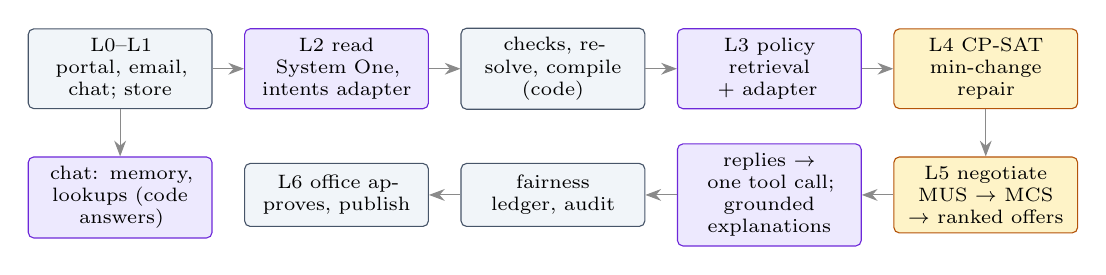
\begin{tikzpicture}[font=\scriptsize, node distance=3mm and 4mm,
  m/.style={draw=modelline, fill=modelfill, rounded corners=2pt, align=center, minimum height=8mm, text width=2.1cm},
  c/.style={draw=codeline, fill=codefill, rounded corners=2pt, align=center, minimum height=8mm, text width=2.1cm},
  s/.style={draw=solverline, fill=solverfill, rounded corners=2pt, align=center, minimum height=8mm, text width=2.1cm},
  a/.style={-{Stealth[length=2mm]}, draw=greyline}]
\node[c] (in) {L0--L1\\portal, email, chat; store};
\node[m, right=of in] (rd) {L2 read\\System One, intents adapter};
\node[c, right=of rd] (ck) {checks, resolve, compile\\(code)};
\node[m, right=of ck] (pol) {L3 policy\\retrieval + adapter};
\node[s, right=of pol] (sv) {L4 CP-SAT\\min-change repair};
\node[s, below=6mm of sv] (ng) {L5 negotiate\\MUS $\to$ MCS $\to$ ranked offers};
\node[m, left=of ng] (rp) {replies $\to$ one tool call; grounded explanations};
\node[c, left=of rp] (fa) {fairness ledger, audit};
\node[c, left=of fa] (ap) {L6 office approves, publish};
\node[m, below=6mm of in] (chat) {chat: memory, lookups (code answers)};
\draw[a] (in) -- (rd); \draw[a] (rd) -- (ck); \draw[a] (ck) -- (pol); \draw[a] (pol) -- (sv);
\draw[a] (sv) -- (ng); \draw[a] (ng) -- (rp); \draw[a] (rp) -- (fa); \draw[a] (fa) -- (ap);
\draw[a] (in) -- (chat);
\end{tikzpicture}
\caption{The request pipeline. Violet: a fine-tuned model reads or writes language; grey: deterministic code;
amber: the constraint solver. Requests made with clicks skip reading entirely.}
\label{fig:arch}
\end{figure}

\noindent A request moves through fixed states (received, classified, policy-checked, compiled, solved, negotiating,
fairness-audited, awaiting approval, published; or answered, forwarded, refused, denied, escalated, clarification
requested, withdrawn); an illegal transition raises an error. Every model-backed component has a deterministic
stand-in (a rule parser, a rule-based policy check, a regex question reader, template explanations), so the system
keeps working, more weakly, when the model server is away; requests that would change the timetable wait up to ten
minutes for the model rather than be read by the stand-in.

\begin{figure}[H]
\centering
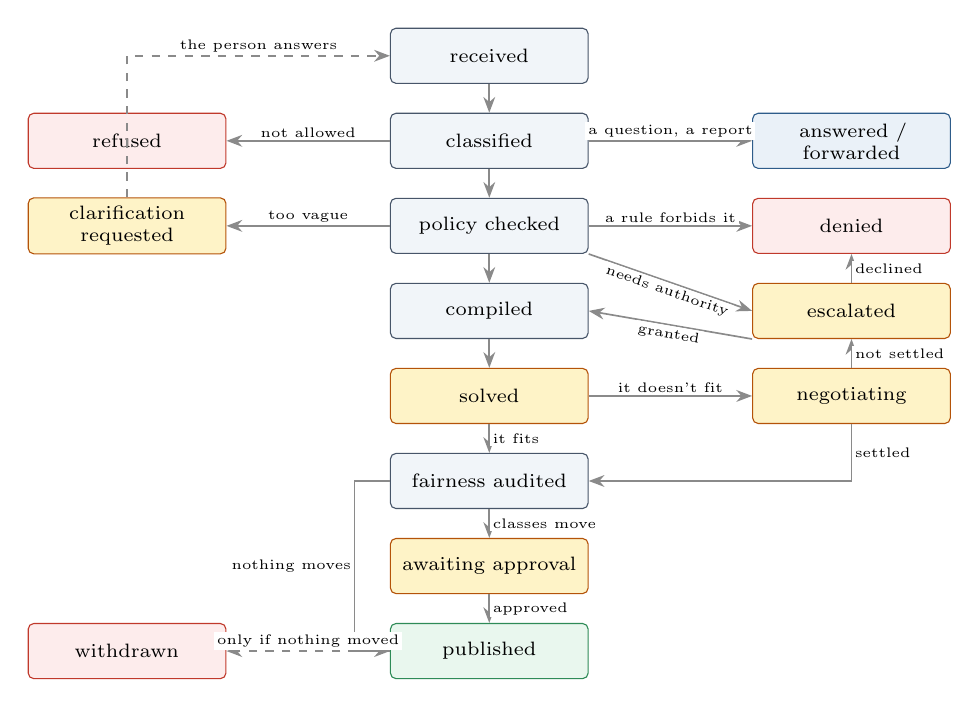
\begin{tikzpicture}[x=1cm, y=1.08cm]
\tikzset{st/.style={bx, text width=2.3cm, minimum height=6.5mm}}
% the normal path, straight down
\node[st, cde] (rcv) at (0,0) {received};
\node[st, cde] (cls) at (0,-1) {classified};
\node[st, cde] (pol) at (0,-2) {policy checked};
\node[st, cde] (cmp) at (0,-3) {compiled};
\node[st, slv] (sol) at (0,-4) {solved};
\node[st, cde] (fai) at (0,-5) {fairness audited};
\node[st, slv] (awa) at (0,-6) {awaiting approval};
\node[st, okb] (pub) at (0,-7) {published};
% exits to the left
\node[st, bad] (ref) at (-4.6,-1) {refused};
\node[st, slv] (cla) at (-4.6,-2) {clarification requested};
\node[st, bad] (wdr) at (-4.6,-7) {withdrawn};
% exits to the right
\node[st, ppl] (ans) at (4.6,-1) {answered / forwarded};
\node[st, bad] (den) at (4.6,-2) {denied};
\node[st, slv] (esc) at (4.6,-3) {escalated};
\node[st, slv] (neg) at (4.6,-4) {negotiating};
\draw[arr] (rcv) -- (cls); \draw[arr] (cls) -- (pol); \draw[arr] (pol) -- (cmp); \draw[arr] (cmp) -- (sol);
\draw[arr] (sol) -- node[lb, right]{it fits} (fai);
\draw[arr] (fai) -- node[lb, right]{classes move} (awa);
\draw[arr] (awa) -- node[lb, right]{approved} (pub);
\draw[arr] (fai.west) -- ++(-0.45,0) |- node[lb, pos=0.25, left]{nothing moves} (pub.west);
\draw[arr] (cls) -- node[lb, above]{not allowed} (ref);
\draw[arr] (cls) -- node[lb, above]{a question, a report} (ans);
\draw[arr] (pol) -- node[lb, above]{too vague} (cla);
\draw[darr] (cla.north) -- ++(0,0.75) |- node[lb, pos=0.75, above]{the person answers} (rcv.west);
\draw[arr] (pol) -- node[lb, above]{a rule forbids it} (den);
\draw[arr] (pol.south east) -- node[lb, below, sloped]{needs authority} (esc.west);
\draw[arr] (esc) -- node[lb, right]{declined} (den);
\draw[arr] (esc.south west) -- node[lb, below, sloped]{granted} (cmp.east);
\draw[arr] (sol) -- node[lb, above]{it doesn't fit} (neg);
\draw[arr] (neg) -- node[lb, right]{not settled} (esc);
\draw[arr] (neg.south) |- node[lb, pos=0.25, right]{settled} (fai.east);
\draw[darr] (pub) -- node[lb, above]{only if nothing moved} (wdr);
\end{tikzpicture}
\caption{A request's life. Only these transitions are allowed. Amber: waiting on a person or the solver; green: in
force; red: it stops; blue: answered or passed on.}
\label{fig:life}
\end{figure}

\subsection{Reading requests (L2)}
\label{sec:method-read}
A message is first prepared: lines that instruct the system are removed before any reader sees them (a message that
is nothing else is refused unread), and shorthand is spelled out (``pls shift my DBMS lec'' becomes ``please shift
my Database Systems lecture''). \textbf{System One}, a calibrated linear SVM over TF-IDF features, routes it. While
the model server is up, the fine-tuned \textbf{intents adapter} reads every request into an \texttt{IntentOutput}:
an action (compile, clarify, investigate, answer, out of scope, withdraw) and intents in 17 kinds (unavailable,
avoid, only, move, swap, extra class, cancel, room closed, needs room, load limit, limit, relate, any-of, ranked,
fallback, club booking, clash report). The model writes clock times (``after 14:00''), periods (\texttt{next\_week})
and class descriptions (``my Monday Data Structures lecture''), never slot numbers or IDs. Code then checks the
reading against the message and the timetable (repairing near misses, turning a hedged requirement into a wish and a
contradiction into a question), resolves names, times, weeks and classes, assigns \textbf{priority tiers} by rule
(0 physical, 1 policy, 2 commitment, 3 verified unavailability, 4 operational, 5 preference), checks authority, and
compiles constraints. Any part of a message the reading did not use is reported back to the sender.

\begin{bluebox}{Worked example: from a message to a constraint}
\small
\textbf{Message} (a teacher, through the portal): \emph{``pls shift my DBMS lec frm monday to thursday afternoon if
possible''}

\textbf{1. Prepared.} Shorthand spelled out: ``please shift my Database Systems lecture from Monday to Thursday
afternoon if possible''.

\textbf{2. Read by the intents adapter} (the model's whole output):
\begin{verbatim}
{"action": "compile", "intents": [{"kind": "move",
  "which": {"course": "Database Systems", "kind": "lecture", "day": "Mon"},
  "to": {"days": ["Thu"], "part": "afternoon"}, "hard": false}]}
\end{verbatim}
\textbf{3. Checked and resolved by code.} ``Database Systems'' is found in the department's courses; ``my \ldots\ lecture
on Monday'' is matched to the one session the teacher holds on Monday in the published timetable; ``afternoon''
becomes the slots from 14:00 to 16:00 on the calendar; no period given means every week; ``if possible'' agrees
with \texttt{hard: false}, so it stays a wish.

\textbf{4. Compiled.} A preference (Tier 5) that this session be placed on Thursday afternoon, owned by the
teacher, with authority checked (it is their own class). The policy check then finds no rule against it, and the
solver repairs the week.
\end{bluebox}

\subsection{Policy check (L3)}
The top five rules are retrieved by hybrid search (BM25 and bge-small embeddings, fused by reciprocal rank) over the
handbook and policy documents in any form (PDF, OCR of scans and photos, HTML). The policy adapter returns a verdict
(allowed, needs approval, forbidden), cited rules, obligations such as a make-up class, and an alternative. Code
then drops any citation of a rule it was not shown, and \textbf{nothing is denied without the rule it breaks}: an
uncited denial becomes ``needs approval''. The examination regulations are applied by code.

\subsection{Solving and negotiation (L4--L5)}
\label{sec:method-neg}
\textbf{Solver.} CP-SAT places every class once with no clash and a fitting room (Tier 0, always enforced). Every
other firm constraint $C_k$ is guarded by an assumption literal ($a_k \Rightarrow C_k$), so conflict analysis can
switch constraints off; wishes and, in repair mode, moved classes form the objective, solved tier by tier. A repair
may be restricted to the neighbourhood a conflict touches.

\textbf{Priority.} Within a tier each constraint has a published score
$\pi_k = w_1\,\mathit{auth} + w_2\,\mathit{impact} + w_3\,\mathit{just} + w_4\,\mathit{lead} + w_5\,\mathit{credit}
- w_6\,\mathit{disrupt}$, and a correction option $M$ costs
$\mathrm{cost}(M) = \sum_{k\in M}\pi_k + \lambda_1\,\mathrm{disruption}(M) + \lambda_2\,\Delta\mathrm{Gini}(M)$,
where $\Delta\mathrm{Gini}$ is the change in how unevenly the concession burden falls.

\textbf{The resolution ladder.} (1) \emph{Auto-substitute}: if the firm constraints fit together, repair and
notify. (2) \emph{Auto-relax}: wishes the repair cannot keep are dropped and their owners told. (3) \emph{Negotiate}:
find the MUS, enumerate MCSs within the relaxable tiers, each with a solver-found witness timetable, rank them by
cost, and ask the owner of the cheapest with two or three verified options and a grounded explanation; a declined
option rules out its day and part of day for the next offers, and a counter-offer is passed on only if CP-SAT
verifies it. (4) \emph{Escalate} on deadlock, no reply, the round limit, or a conflict only a Tier 1--2 authority can
relax. Each reply becomes \textbf{exactly one typed tool call} (accept, apply reply, counter-propose, ask
clarification, decline, escalate); the ladder, not the model, decides what it does.

\begin{figure}[H]
\centering
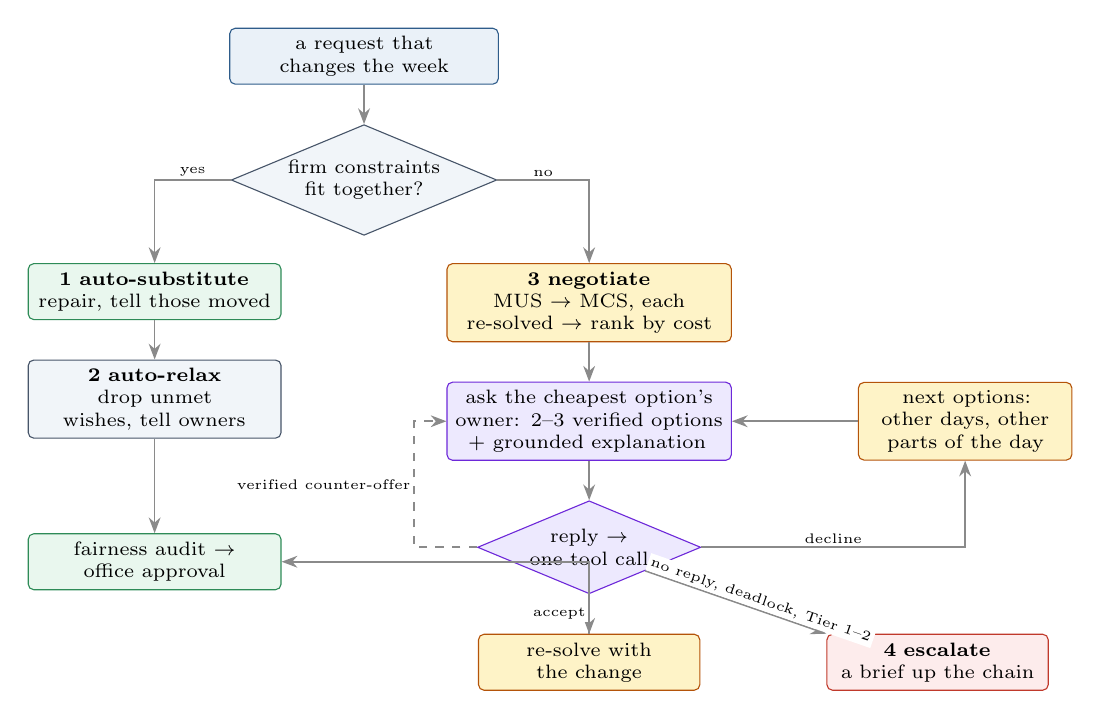
\begin{tikzpicture}[node distance=5mm and 6mm]
\node[ppl, text width=3.2cm] (req) {a request that changes the week};
\node[dec, below=of req] (fit) {firm constraints\\fit together?};
\node[okb, text width=3.0cm, below left=7mm and 2mm of fit] (sub) {\textbf{1 auto-substitute}\\repair, tell those moved};
\node[cde, text width=3.0cm, below=of sub] (rlx) {\textbf{2 auto-relax}\\drop unmet wishes, tell owners};
\node[slv, text width=3.4cm, below right=7mm and 2mm of fit] (neg) {\textbf{3 negotiate}\\MUS $\to$ MCS, each re-solved $\to$ rank by cost};
\node[mdl, text width=3.4cm, below=of neg] (ask) {ask the cheapest option's owner: 2--3 verified options + grounded explanation};
\node[decm, below=of ask] (rep) {reply $\to$\\one tool call};
\node[slv, text width=2.5cm, right=16mm of ask] (nxt) {next options: other days, other parts of the day};
\node[slv, text width=2.6cm, below=of rep] (rs) {re-solve with the change};
\node[bad, text width=2.6cm, right=16mm of rs] (esc) {\textbf{4 escalate}\\a brief up the chain};
\node[okb, text width=3.0cm, below=12mm of rlx] (done) {fairness audit $\to$ office approval};
\draw[arr] (req) -- (fit);
\draw[arr] (fit) -| node[lb, above, pos=0.25]{yes} (sub);
\draw[arr] (fit) -| node[lb, above, pos=0.25]{no} (neg);
\draw[arr] (sub) -- (rlx); \draw[arr] (rlx) -- (done);
\draw[arr] (neg) -- (ask); \draw[arr] (ask) -- (rep);
\draw[arr] (rep) -- node[lb, left]{accept} (rs);
\draw[arr] (rep.east) -| node[lb, pos=0.25, above]{decline} (nxt.south);
\draw[arr] (nxt) -- (ask);
\draw[arr] (rep.south east) -- node[lb, sloped, above, pos=0.62]{no reply, deadlock, Tier 1--2} (esc.north west);
\draw[arr] (rs) |- (done);
\draw[darr] (rep.west) -- ++(-0.8,0) |- node[lb, pos=0.25, left]{verified counter-offer} (ask.west);
\end{tikzpicture}
\caption{The resolution ladder. The solver decides what may be offered; the model only explains the offers and reads
the replies.}
\label{fig:ladder}
\end{figure}

\begin{bluebox}{Worked example: two practicals, one GPU lab (illustrative)}
\small
Two teachers ask for the only GPU lab on Thursday afternoon. \textbf{The MUS} is the two requests plus the lab's
capacity: remove any one and the week fits. \textbf{The MCSs}, each re-solved into a full timetable, are, for example,
(a) the first practical moves to Friday 14:00 in the GPU lab, (b) the second moves to Tuesday 11:00, or (c) the first
stays on Thursday in a lab without GPUs. Ranked by cost (the owner's tier, scores and concession history, and how many
other classes move), the cheapest option's owner is asked first, with options (a) and (b) and an explanation built
from the facts (``Lab 3 is the only lab with GPUs; both practicals were requested for Thursday 14:00--17:00''),
never from the other teacher's private reason. If the owner declines, the next options avoid Friday afternoon; if
they accept, the week is re-solved with the change and sent to the office for approval.
\end{bluebox}

\textbf{Explanations} are built from numbered facts (the constraints in the conflict, the rules, the verified
options, the ledger) that name constraints, never private reasons; the model writes claims citing fact IDs, and a
checker drops any claim that cites nothing or mentions a day, number or name absent from its facts.
\textbf{The concession ledger} credits each accepted concession by $\mathrm{importance}\times\mathrm{magnitude}$,
lowers the chance of asking the same person again, and decays each semester. \textbf{Approval}: every change that
moves a class waits for the timetable office.

\subsection{The chat: timetable questions and memory}
\label{sec:method-chat}
A lookup adapter chooses \emph{what} to look up; 16 lookup tools compute the answer from the week's timetable and the
records (free hours, classes, free rooms, who is free, changes, the calendar, the asker's requests and rules,
clashes, move options, counts, gaps, fairness, bookings, a what-if dry run). The model writes names as the message
writes them; code resolves them, roles included (``the HOD'' is whoever holds the role today), and every choice is
checked, with a problem sent back to the model at most three times. Four generations were built:
\textbf{v1} (one lookup, names listed in the prompt), \textbf{v2} (roles, shared courses), \textbf{v3} (up to five
lookups and ten new tools, names as written; in use) and \textbf{v4}, a typed \emph{lookup vocabulary} like the
request one: a part per thing asked, each tool with only its own fields, clock times and periods instead of slots and
week numbers, and request and rule parts that keep their own words. A message mixing questions, a rule question and
a request is answered part by part: questions from the timetable, the rule question from the handbook, and the
request sent into the pipeline.

\textbf{Memory} runs first: given the newest message and the four before it, the memory adapter answers
\texttt{\{"same"\}}, the message rewritten to stand alone, or a question back, and a rewrite may name only what the
conversation names. \textbf{Memory v2} fills a request from the answer in the \emph{same} message (``when am I free on
Friday? move my DS lecture there''), and asks which time when the answer has several.

\begin{figure}[H]
\centering
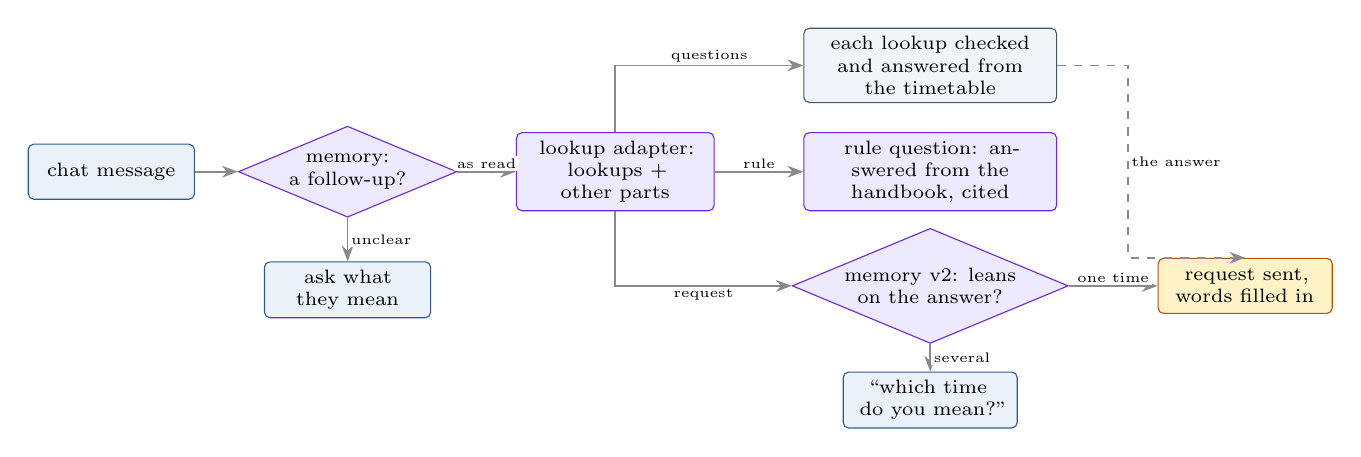
\begin{tikzpicture}[x=1cm, y=1cm]
\node[ppl, text width=1.9cm] (msg) at (0,0) {chat message};
\node[decm] (mem) at (3.0,0) {memory:\\a follow-up?};
\node[ppl, text width=1.9cm] (ab) at (3.0,-1.5) {ask what they mean};
\node[mdl, text width=2.3cm] (rd) at (6.4,0) {lookup adapter: lookups + other parts};
\node[cde, text width=3.0cm] (q) at (10.4,1.35) {each lookup checked and answered from the timetable};
\node[mdl, text width=3.0cm] (rl) at (10.4,0) {rule question: answered from the handbook, cited};
\node[decm] (v2) at (10.4,-1.45) {memory v2: leans\\on the answer?};
\node[slv, text width=2.0cm] (snd) at (14.4,-1.45) {request sent, words filled in};
\node[ppl, text width=2.0cm] (wh) at (10.4,-2.9) {``which time do you mean?''};
\draw[arr] (msg) -- (mem); \draw[arr] (mem) -- node[lb, above]{as read} (rd);
\draw[arr] (mem) -- node[lb, right]{unclear} (ab);
\draw[arr] (rd.north) |- node[lb, pos=0.75, above]{questions} (q.west);
\draw[arr] (rd) -- node[lb, above]{rule} (rl);
\draw[arr] (rd.south) |- node[lb, pos=0.75, below]{request} (v2.west);
\draw[arr] (v2) -- node[lb, above]{one time} (snd);
\draw[arr] (v2) -- node[lb, right]{several} (wh);
\draw[darr] (q.east) -- ++(0.9,0) |- node[lb, pos=0.25, right]{the answer} (snd.north);
\end{tikzpicture}
\caption{One chat message with questions, a rule question and a request. The model chooses what to look up; code
answers from the timetable.}
\label{fig:chat}
\end{figure}

\begin{bluebox}{Worked example: the same message in lookup v3 and in the lookup vocabulary (v4)}
\small
\emph{``is Khan sir free Thu after lunch? also move my DS lecture there''}

\textbf{v3} (flat choices; the model counts slots and weeks, and the request is a wordless \texttt{none}):
\begin{verbatim}
{"lookups": [{"tool": "free_hours", "teachers": ["khan sir"], "days": ["Thu"],
              "hours": [5, 6, 7], "week": 15},
             {"tool": "none", "week": 15}]}
\end{verbatim}
\textbf{v4} (a part per thing asked, clock times, the request keeps its words):
\begin{verbatim}
{"parts": [{"tool": "free_hours", "who": {"teachers": ["khan sir"]},
            "when": {"days": ["Thu"], "after": "14:00"}},
           {"tool": "request", "text": "move my DS lecture there"}]}
\end{verbatim}
In both, code finds who ``Khan sir'' is and answers from the timetable. With v4, memory v2 then rewrites the request
part from the answer (``move my Data Structures lecture to Thursday 2--3\,pm''), which v3 cannot, since its request
part has no words.
\end{bluebox}

\subsection{The coordinator agent}
\label{sec:method-agent}
As an alternative to the fixed pipeline, a tool-calling coordinator works a whole request through about 30 typed tools in five scopes: read the department, draft changes, check the draft
(a repair solve of every affected week), talk to people (ask the requester, offer a waiver to the owner of a blocking
rule), and end (submit, decline, escalate). Only a commit gate changes state, re-checking every change with the
validator whatever the agent claimed, so every model mistake becomes an error the model sees rather than a bad
timetable. Traces are labelled by the scenario's verdict or the office's approval and exported for SFT, and as DPO
pairs (a refused turn against its fix; a good against a bad episode of the same request).

\begin{figure}[H]
\centering
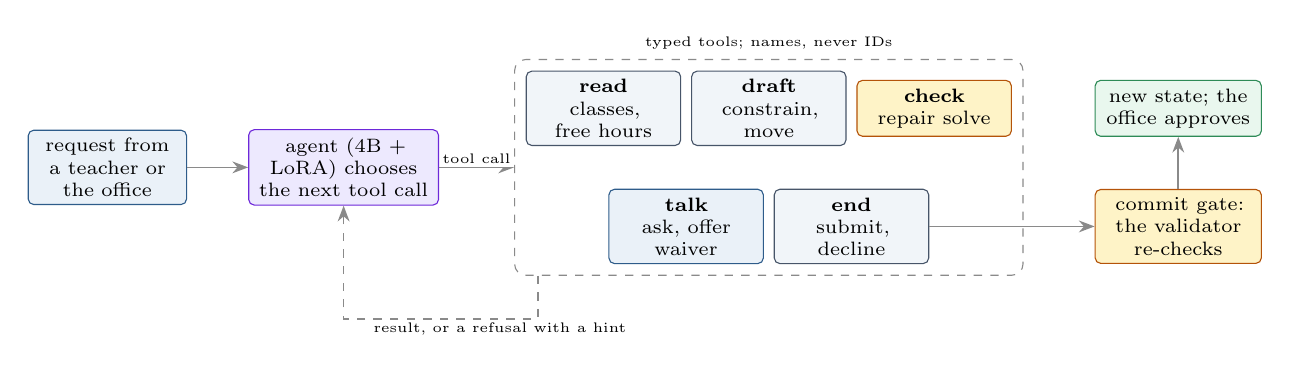
\begin{tikzpicture}[x=1cm, y=1cm]
\node[ppl, text width=1.8cm] (rq) at (0,0) {request from a teacher or the office};
\node[mdl, text width=2.2cm] (ag) at (3.0,0) {agent (4B + LoRA) chooses the next tool call};
\node[cde, text width=1.75cm] (rdt) at (6.3,0.75) {\textbf{read}\\classes, free hours};
\node[cde, text width=1.75cm] (drf) at (8.4,0.75) {\textbf{draft}\\constrain, move};
\node[slv, text width=1.75cm] (chk) at (10.5,0.75) {\textbf{check}\\repair solve};
\node[ppl, text width=1.75cm] (tlk) at (7.35,-0.75) {\textbf{talk}\\ask, offer waiver};
\node[cde, text width=1.75cm] (end) at (9.45,-0.75) {\textbf{end}\\submit, decline};
\begin{scope}[on background layer]
\node[draw=greyline, dashed, rounded corners, fit=(rdt)(chk)(tlk)(end), inner sep=4pt,
  label={[font=\tiny]above:typed tools; names, never IDs}] (tools) {};
\end{scope}
\node[slv, text width=1.9cm] (gate) at (13.6,-0.75) {commit gate: the validator re-checks};
\node[okb, text width=1.9cm] (st) at (13.6,0.75) {new state; the office approves};
\draw[arr] (rq) -- (ag);
\draw[arr] (ag) -- node[lb, above]{tool call} (tools.west);
\draw[darr] (tools.south west) ++(0.3,0) |- ++(-2.4,-0.55) node[lb, below, pos=0.6]{result, or a refusal with a hint} -| (ag.south);
\draw[arr] (end) -- (gate); \draw[arr] (gate) -- (st);
\end{tikzpicture}
\caption{The coordinator agent's loop. The model never writes the timetable: only the commit gate changes state, and
every refused call becomes feedback the model sees on its next turn.}
\label{fig:agent}
\end{figure}

\subsection{Fine-tuning}
\label{sec:method-ft}
\textbf{One base, an adapter per task.} Qwen3.5-4B (Q8\_0 GGUF) is served once by \texttt{llama-server} with every
adapter loaded at scale zero; each call switches on its task's adapter. Each adapter is retrained and evaluated
alone, so a change to the chat never puts request reading at risk.

\textbf{Which layers, and why.} Every adapter uses rank 16, $\alpha=16$, no dropout, on the linear layers named
\texttt{q/k/v/o\_proj} and \texttt{gate/up/down\_proj} outside the vision tower. Qwen3.5 is a hybrid: of its 32 layers,
24 use Gated DeltaNet linear attention and every fourth uses full attention. The pattern therefore adapts the full
attention of 8 layers (3.1M weights) and the MLP of all 32 (18.1M), about 21M weights or 0.5\% of the model; the
linear-attention projections, embeddings, output head and vision tower stay frozen. Full fine-tuning would need
roughly four times the 17\,GB fp32 model in memory, beyond two 15\,GB T4s. Attention is adapted because our tasks are
mostly \emph{finding and copying} the right words of the prompt; the MLPs because the model must \emph{transform}
phrases into a vocabulary it never saw, and adapting all linear layers is the standard LoRA practice. Embeddings and output head are frozen because no new tokens are needed and their shared matrix
(636M weights) would make each adapter larger than a gigabyte. Leaving out the linear-attention layers was a side
effect of a name pattern written for ordinary transformers, not a choice (Section~\ref{sec:limits}).

\begin{figure}[H]
\centering
\begin{minipage}[t]{0.47\textwidth}\centering
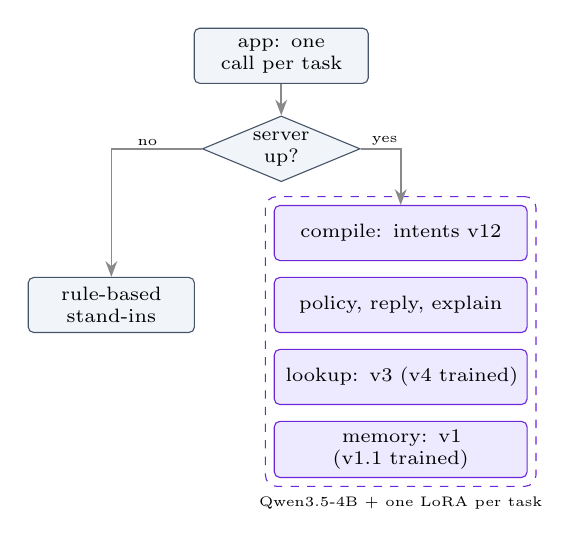
\begin{tikzpicture}[node distance=3mm and 4mm]
\node[cde, text width=2.0cm] (app) {app: one call per task};
\node[dec, below=4mm of app] (ml) {server\\up?};
\node[mdl, text width=3.0cm, below right=5mm and -6mm of ml] (a1) {compile: intents v12};
\node[mdl, text width=3.0cm, below=2mm of a1] (a2) {policy, reply, explain};
\node[mdl, text width=3.0cm, below=2mm of a2] (a3) {lookup: v3 (v4 trained)};
\node[mdl, text width=3.0cm, below=2mm of a3] (a4) {memory: v1 (v1.1 trained)};
\node[cde, text width=1.9cm, left=10mm of a2] (fb) {rule-based stand-ins};
\begin{scope}[on background layer]
\node[draw=modelline, dashed, rounded corners, fit=(a1)(a4), inner sep=3pt,
  label={[font=\tiny]below:Qwen3.5-4B + one LoRA per task}] {};
\end{scope}
\draw[arr] (app) -- (ml);
\draw[arr] (ml) -| node[lb, above, pos=0.3]{yes} (a1.north);
\draw[arr] (ml) -| node[lb, above, pos=0.3]{no} (fb.north);
\end{tikzpicture}
\end{minipage}\hfill
\begin{minipage}[t]{0.47\textwidth}\centering
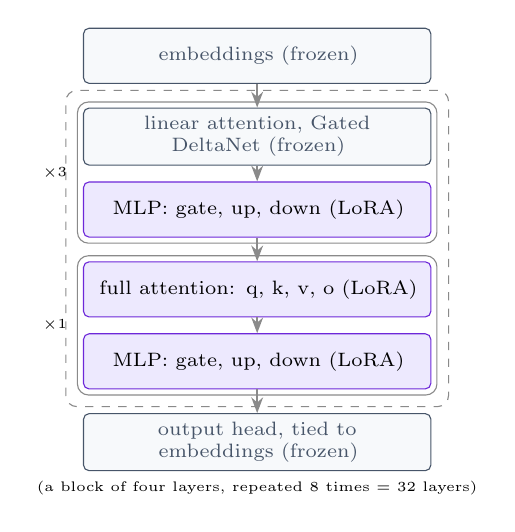
\begin{tikzpicture}[node distance=2mm]
\node[cde, text width=4.2cm, fill=codefill!60, text=codeline] (emb) {embeddings (frozen)};
\node[cde, text width=4.2cm, fill=codefill!60, text=codeline, below=3mm of emb] (la) {linear attention, Gated DeltaNet (frozen)};
\node[mdl, text width=4.2cm, below=of la] (m1) {MLP: gate, up, down (LoRA)};
\node[mdl, text width=4.2cm, below=3mm of m1] (fa) {full attention: q, k, v, o (LoRA)};
\node[mdl, text width=4.2cm, below=of fa] (m2) {MLP: gate, up, down (LoRA)};
\node[cde, text width=4.2cm, fill=codefill!60, text=codeline, below=3mm of m2] (hd) {output head, tied to embeddings (frozen)};
\begin{scope}[on background layer]
\node[draw=greyline, rounded corners, fit=(la)(m1), inner sep=2pt, label={[font=\tiny]left:$\times 3$}] (b1) {};
\node[draw=greyline, rounded corners, fit=(fa)(m2), inner sep=2pt, label={[font=\tiny]left:$\times 1$}] (b2) {};
\node[draw=greyline, dashed, rounded corners, fit=(b1)(b2), inner sep=4pt] (blk) {};
\node[font=\tiny, anchor=north] at (hd.south) {(a block of four layers, repeated 8 times = 32 layers)};
\end{scope}
\draw[arr] (emb) -- (la); \draw[arr] (la) -- (m1); \draw[arr] (m1) -- (fa); \draw[arr] (fa) -- (m2);
\draw[arr] (m2) -- (hd);
\end{tikzpicture}
\end{minipage}
\caption{Left: one base model serves every task, an adapter switched on per call, with rule-based stand-ins when the
server is away. Right: which layers the adapters train (violet): the MLP of all 32 layers and the attention of the 8
full-attention layers, about 21M weights (0.5\% of the model).}
\label{fig:lora}
\end{figure}

\textbf{Training.} Loss is on the answer only; the prompt is masked. Learning rate $2\times10^{-4}$ for a new adapter
and $5\times10^{-5}$ when continuing from the previous version (with part of its rows replayed), cosine schedule.
The lookup and memory adapters train one epoch in fp32 (fp16 overflowed on the T4s, which lack bf16); the intents
adapter trains three epochs in fp16 with the loss scale started at $2^8$, saving the adapter at a third, two thirds
and all of its rows (\texttt{read-033/067/100}). Adapters are exported as LoRA GGUF files of tens of MB.

\begin{table}[H]
\centering\small
\begin{tabularx}{\textwidth}{@{}L{3.2cm} L{4.6cm} Y@{}}
\toprule
\textbf{Setting} & \textbf{Value} & \textbf{Why}\\
\midrule
Rank, alpha & 16, 16 & Narrow tasks need little capacity; $\alpha/r=1$ keeps the learning rate's meaning fixed\\
Dropout, bias & 0, none & One pass over varied generated rows gives little to overfit\\
Loss & On the answer only & The prompt is given at run time; learning it would teach one department's details\\
Learning rate & $2\times10^{-4}$ new; $5\times10^{-5}$ continuing & Continue from the previous adapter without overwriting it\\
Schedule & Cosine, 5 warm-up steps & A gentle start, decaying to zero\\
Precision & fp32 (lookup, memory); fp16, loss scale $2^8$ (intents) & T4s lack bf16; plain fp16 overflowed (\texttt{nan} gradients)\\
Max length, batch & 2,048 tokens, 1 row (lookup, memory); 512 tokens, 16 rows (intents) & Lookup rows are 900--1,300 tokens with the prompt; intents rows under 300\\
Epochs & 1 (lookup, memory); 3 (intents) & More passes memorise wordings; the third intents epoch teaches the smallest skills\\
\bottomrule
\end{tabularx}
\caption{Training settings, shared by every adapter except where stated.}
\label{tab:hparams}
\end{table}

\textbf{Training data.} No real user's messages were used. Every row is generated from a known answer, or reworded
by Gemini and kept only if reading it back gives the same answer, and every row passes the same gates whatever its
source (Figure~\ref{fig:data}). The request reader's test split is frozen by a fingerprint, so every version is
scored on the same 417 requests, and test templates and wordings never appear in training.

\begin{figure}[H]
\centering
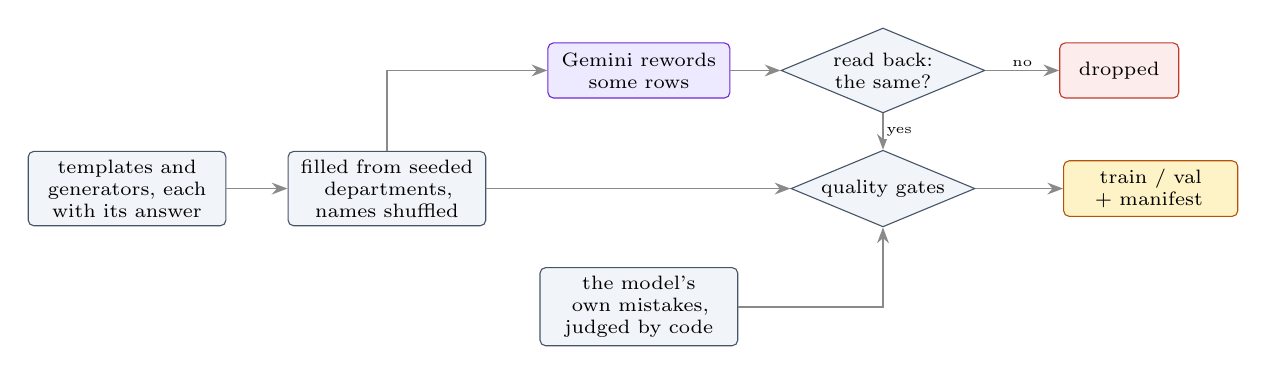
\begin{tikzpicture}[x=1cm, y=1cm]
\node[cde, text width=2.3cm] (tpl) at (0,0) {templates and generators, each with its answer};
\node[cde, text width=2.3cm] (fill) at (3.3,0) {filled from seeded departments, names shuffled};
\node[mdl, text width=2.1cm] (gem) at (6.5,1.5) {Gemini rewords some rows};
\node[dec] (bk) at (9.6,1.5) {read back:\\the same?};
\node[bad, text width=1.3cm] (drop) at (12.6,1.5) {dropped};
\node[cde, text width=2.3cm] (mine) at (6.5,-1.5) {the model's own mistakes, judged by code};
\node[dec] (gate) at (9.6,0) {quality gates};
\node[slv, text width=2.0cm] (out) at (13.0,0) {train / val + manifest};
\draw[arr] (tpl) -- (fill); \draw[arr] (fill) -- (gate);
\draw[arr] (fill.north) |- (gem.west); \draw[arr] (gem) -- (bk);
\draw[arr] (bk) -- node[lb, above]{no} (drop); \draw[arr] (bk) -- node[lb, right]{yes} (gate);
\draw[arr] (mine.east) -| (gate.south); \draw[arr] (gate) -- (out);
\end{tikzpicture}
\caption{How training rows are made. Every source passes the same gates; the test split and test wordings are kept
apart.}
\label{fig:data}
\end{figure}

% ==================================================================
\section{Experiment Runs}
\label{sec:runs}
% ==================================================================
\begin{table}[H]
\centering\small
\begin{tabularx}{\textwidth}{@{}L{3.6cm} Y L{3.6cm}@{}}
\toprule
\textbf{Experiment} & \textbf{What was run} & \textbf{Models}\\
\midrule
Main negotiation & Ours, B3, B4: 60 scenarios $\times$ 3 seeds (180 paired runs each); A1--A3: stratified 30, seed 0; B1: stratified 20; B2 and oracle: all 60 (no model); offline replica of ours, A1 and B2 & Ours: Qwen3.5-4B + LoRA; baselines: Gemini 3.5 Flash-Lite; simulators: model-voiced\\
Request reading & 151-request compile test; 417-request frozen intent test; 26 held-out suites; v6--v13 & Rule parser, Gemini, 2B/4B LoRA, intents v6--v13 at each curve point\\
Policy, retrieval & Allow/deny, citations, obligations; recall@1/3/5 and MRR for three retrievers & Gemini, 4B LoRA; BM25, dense, hybrid\\
Replies, safety & 100 replies; 48--50 safety cases through the real pipeline, also with a parser that obeys every injection & Base 4B, Gemini, 4B LoRA, regex\\
Timetable questions & Sets A, B2, B3, C, D (362 each); new-kind sets; 200 long messages; 26 chat cases through the app & Regex, Gemini, lookup v1--v4, v3.2\\
Memory & 400 test conversations, memory then lookup; 64 plural conversations; 8 memory-v2 chat cases & Memory v1 (v1.1 trained)\\
Agent & 49--50 families $\times$ 10 episodes over two departments; best-of-$n$; held-out rewritten requests & Base 4B, Gemini, agent v3--v7 (SFT, DPO)\\
\bottomrule
\end{tabularx}
\caption{Experiment runs. Every model answer is cached by model and prompt, so any table can be re-scored without
model calls and interrupted runs resume.}
\end{table}

\noindent\textbf{Compute.} Training ran on free Kaggle sessions (two T4 GPUs, 12-hour limit; runs resume from
checkpoints): a lookup or memory adapter takes 3--4 hours, an intents version one session. Serving and evaluation
used one shared GPU machine running \texttt{llama-server}; the solver runs on CPU. Gemini was used for baselines,
simulators, rewordings and the judge, within free-tier quotas.

\subsection{Configurations compared in the main experiment}
Table~\ref{tab:configs} lists every configuration of the main experiment, and the question each one answers.
\begin{table}[!htb]
\centering\small
\begin{tabularx}{\textwidth}{@{}L{2.6cm} Y L{4.4cm}@{}}
\toprule
\textbf{Configuration} & \textbf{What it does} & \textbf{Question it answers}\\
\midrule
\textbf{Ours} & MCS options, each re-solved; tiers and ledger; grounded explanations; replies read as typed tool calls & The system under test\\
B1 LLM only & The model writes the timetable directly; no solver & Can a model just do it?\\
B2 Solver only & Same solver, tiers and objective, but the cheapest repair is imposed without asking anyone & Is negotiation needed, or only a solver?\\
B3 Unverified & As ours, but the model invents the options and they are offered unchecked & How often are invented options infeasible?\\
B4 Filtered & As B3, but CP-SAT drops infeasible inventions and the model tries again (up to 3 calls a round) & The strongest ``model invents'' system (primary baseline)\\
Oracle & CP-SAT with every stakeholder's hidden flexibility & The best possible outcome (upper bound)\\
A1 / A2 / A3 & Ours with flat weights / free-text explanations / a regex reply reader & What each part contributes (Section~\ref{sec:ablations})\\
\bottomrule
\end{tabularx}
\caption{Configurations of the main experiment.}
\label{tab:configs}
\end{table}

\subsection{Metrics}
\begin{itemize}
\item \textbf{Correct outcome}: the run ends as the oracle's does (an agreement, or an escalation where none is
possible). A scenario is \emph{resolved} when every affected stakeholder accepted an offered alternative and the
combined repair re-solves feasibly.
\item \textbf{Agreement}: the run ends in an agreement rather than an escalation. \textbf{Rounds}: rounds of messages
before it ends.
\item \textbf{Oracle gap}: how much worse the final timetable is than the oracle's, by the oracle's own objective
(lower is better).
\item \textbf{Invalid options}: offered options that are infeasible; for B4, how many inventions the solver filtered.
\item \textbf{Fairness}: the Gini coefficient of the weighted concession burden over a ``semester'' of scenarios run
in order with one ledger, and the largest individual burden.
\item \textbf{Explanations}: private-reason leaks, and claim faithfulness (the share of claims traceable to a fact).
\item \textbf{Reading}: \emph{outcome match}, whether a reading leads to the same change to the timetable as the
correct one (a different wording that does the same thing counts as right), and \emph{silently wrong}, a reading
that changes the timetable wrongly without asking. Timetable questions are scored by what each lookup resolves to
after the code resolves names and weeks, not by its wording.
\end{itemize}

\noindent\textbf{Protocol.} Ours, B3 and B4 run the same 60 scenarios with the same three seeds, so runs are paired,
and correct outcomes are compared with McNemar's test. Each scenario carries one stakeholder style, balanced within
each kind of conflict, and replies are random within the style, so no system can succeed by exploiting a fixed reply
rule. Scenarios run in order with one concession ledger per configuration and seed, so the burden builds up as over a
semester among the same people.

% ==================================================================
\section{Evaluations}
\label{sec:eval}
% ==================================================================
\subsection{Main experiment: solver-grounded negotiation}
\label{sec:eval-main}
A run is \emph{correct} when its final status matches the oracle's (the solver with every stakeholder's hidden
flexibility). The baselines use the much larger Gemini 3.5 Flash-Lite, so they are not handicapped on
language.

\begin{table}[H]
\centering\small
\begin{tabularx}{\textwidth}{@{}l c C C C C C@{}}
\toprule
\textbf{System} & \textbf{$n$} & \textbf{Correct outcome} & \textbf{Agreement} & \textbf{Rounds} & \textbf{Oracle gap} & \textbf{Invalid options}\\
\midrule
B1 LLM only & 20 & 0.0\% & 0.0\% & -- & -- & 80\% of timetables\\
B2 Solver only & 60 & 31.7\% & 0.0\% & -- & 0.131 & --\\
B3 Unverified & 180 & 83.3\% & 66.7\% & 1.47 & 0.443 & 51.0\%\\
B4 Filtered & 180 & 75.6\% & 51.1\% & 1.48 & 0.628 & 5.7 filtered/sc.\\
\textbf{Ours} & 180 & \best{89.4\%} & \best{78.9\%} & \best{1.38} & \best{0.041} & \best{0}\\
\bottomrule
\end{tabularx}
\caption{Main results. McNemar's test on correct outcome: ours vs B4 $p=4.6\times10^{-6}$, vs B3
$p=0.013$; differences in rounds are not significant.}
\label{tab:main}
\end{table}

\noindent A model writing the timetable (B1) breaks it every time. A solver alone (B2) finds a valid repair but
imposes it, and is right only a third of the time: hidden flexibility matters, so negotiation is needed. Half of the
options a model invents are infeasible (B3). Filtering them (B4) is \emph{worse} than not filtering: the solver
rejects most inventions, the survivors are fewer and worse, and fewer people agree. Ours offers only feasible
options and lands almost on the oracle (gap 0.04). \textbf{Failures}: 19 of 180 runs, all safe escalations where the
oracle found agreement: a stakeholder did not reply in time (11), or the acceptable option was not among those
offered (8). No run offered an infeasible timetable.

\begin{figure}[H]
\centering
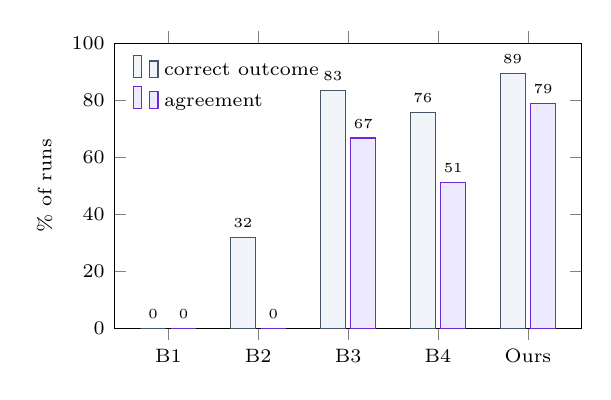
\begin{tikzpicture}
\begin{axis}[
  ybar, bar width=9pt, width=0.62\textwidth, height=5.2cm,
  ymin=0, ymax=100, ylabel={\% of runs}, ylabel style={font=\scriptsize},
  symbolic x coords={B1,B2,B3,B4,Ours}, xtick=data, tick label style={font=\scriptsize},
  legend style={font=\scriptsize, at={(0.02,0.98)}, anchor=north west, draw=none, fill=none},
  legend cell align=left, enlarge x limits=0.15,
  nodes near coords, nodes near coords style={font=\tiny},
  every node near coord/.append style={/pgf/number format/fixed, /pgf/number format/precision=0}]
\addplot[fill=codefill, draw=codeline] coordinates {(B1,0) (B2,31.7) (B3,83.3) (B4,75.6) (Ours,89.4)};
\addplot[fill=modelfill, draw=modelline] coordinates {(B1,0) (B2,0) (B3,66.7) (B4,51.1) (Ours,78.9)};
\legend{correct outcome, agreement}
\end{axis}
\end{tikzpicture}\hfill
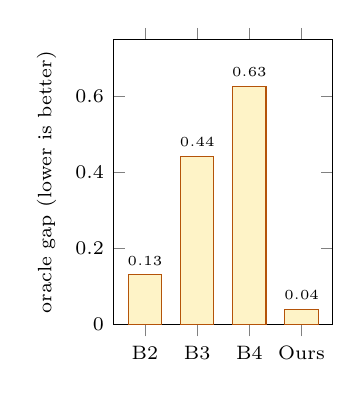
\begin{tikzpicture}
\begin{axis}[
  ybar, bar width=12pt, width=0.36\textwidth, height=5.2cm,
  ymin=0, ymax=0.75, ylabel={oracle gap (lower is better)}, ylabel style={font=\scriptsize},
  symbolic x coords={B2,B3,B4,Ours}, xtick=data, tick label style={font=\scriptsize}, enlarge x limits=0.2,
  nodes near coords, nodes near coords style={font=\tiny},
  every node near coord/.append style={/pgf/number format/fixed, /pgf/number format/precision=2}]
\addplot[fill=solverfill, draw=solverline] coordinates {(B2,0.131) (B3,0.443) (B4,0.628) (Ours,0.041)};
\end{axis}
\end{tikzpicture}
\caption{Main experiment. Left: correct outcome and agreement. Right: distance from the oracle's timetable (B2
imposes a cheap repair, so its gap is small, but it is right only a third of the time).}
\label{fig:main}
\end{figure}

\subsection{What the main results show}
Three things stand out. First, \textbf{verification after the fact is not enough}: filtering invented options (B4)
removes the infeasible ones but leaves fewer and worse offers, so people agree less often than when the unchecked
inventions are offered (B3), and both fall well short of offering verified repairs from the start. Second,
\textbf{the solver alone is not enough either}: imposing the cheapest repair (B2) ignores what people would have
accepted, and is right in under a third of scenarios; asking is what finds the hidden flexibility. Third, \textbf{the
gain does not come from a bigger model}: ours runs on a 4B model against a much larger one for the baselines; the
advantage comes from what the model is allowed to offer. Rounds are statistically equal across systems, so H1 and H2
hold for outcome and quality but not for speed.

\begin{table}[H]
\centering\small
\begin{tabularx}{\textwidth}{@{}l Y l@{}}
\toprule
\textbf{Hyp.} & \textbf{Evidence} & \textbf{Verdict}\\
\midrule
H1 & 51\% of B3's options infeasible; B4 needs 3.97 generation calls per scenario and still agrees least; rounds not significantly higher & \yes{} (rounds n.s.)\\
H2 & Correct 89.4\% vs 75.6\%; oracle gap 0.04 vs 0.63; rounds equal within the confidence interval & \yes{} (except rounds)\\
H3 & Grounded vs free text (A2): 0 vs 12 private-reason leaks; claim faithfulness 0.98, measured automatically & \partly{}\\
H4 & Ledger vs flat weights: Gini 0.241 vs 0.224 (model runs), 0.199 vs 0.224 (offline); one conflict per scenario & \no{}\\
\bottomrule
\end{tabularx}
\caption{Hypotheses.}
\end{table}

\subsection{Component evaluations}
\textbf{Reading requests.} On 151 test requests both fine-tuned models beat the prompted Gemini on compiling
(97.8\% exact against 92.4\%, atom F1 0.996 against 0.977). Scored by \emph{outcome match} (does the reading change
the timetable as the correct one would) on the frozen 417-request split, the rule parser reaches 51.6\% (21.1\%
silently wrong), intents v11 95.4\% (2.4\%), and v12 98.1\% (1.9\%) after its second epoch; the adapter served, after
its third epoch, reaches 96.4\%. On compositional requests (limits, relations, choices) v12 reaches 85.7\% with none
silently wrong.

\textbf{Policy.} The fine-tuned adapter reaches 99\% allow/deny accuracy (Gemini 98\%), deny recall with a cited
rule of 0.90 (0.80), and recall of the make-up class obligation of 1.00 (0.21). Hybrid retrieval reaches recall@5 of
0.93 on corpus requests with the reading's hints.

\textbf{Replies and safety.} On 100 stakeholder replies the fine-tuned adapter reaches 100\% tool and argument
accuracy (prompted base 65\% / 100\%; Gemini 100\% / 85.5\%), with no unsafe action by any reader. Every case of the
safety set is handled safely: no unapproved publish, no authority violation, no injection success, no private leak.

\textbf{Timetable questions and memory.}

\begin{table}[H]
\centering\small
\begin{tabularx}{\textwidth}{@{}Y c c c c c c c@{}}
\toprule
\textbf{Test} & \textbf{Regex} & \textbf{Gemini} & \textbf{v1} & \textbf{v2} & \textbf{v3} & \textbf{v3.2} & \textbf{v4}\\
\midrule
A: app's department (362) & 242 & 320 & 329 & \best{347} & 346 & 339 & 337\\
C: names shuffled (362) & & & 329 & 343 & \best{346}$^*$ & 334 & 340\\
D: unseen, shared courses (360) & & & 327 & \best{345} & 343$^*$ & 335 & 333\\
Long and mixed messages, whole message (200) & & & & & 111 & 119 & \best{140}\\
\quad question parts (561) & & & & & 440 & 445 & \best{483}\\
\quad requests found (123) & & & & & 112 & 117 & \best{122}\\
Chat cases through the app (26) & & & & & 25 & 25 & \best{26}\\
Memory then lookup, end to end (400) & & & & & 387 & 386 & \best{388}\\
\bottomrule
\end{tabularx}
\caption{Timetable questions. $^*$recounted with the current labels (at least); v1 and v2 were scored with the
labels of their time. The adapters score alike across departments: they read rather than memorise.}
\label{tab:lookup}
\end{table}

\textbf{Coordinator agent.} On the 19-family default suite the SFT agent v4 passes 100\% (prompted base 66.7\%,
Gemini 85.1\%), and 100\% of held-out and stress families. On the full 50-family suite over two departments,
agent v6 (SFT then DPO) passes 412/480 (85.8\%), v7 SFT 387/490 (79.0\%) and v7 DPO 381/490 (77.8\%).

% ==================================================================
\section{Ablations}
\label{sec:ablations}
% ==================================================================
An ablation takes the system and removes or replaces exactly one part, or compares two versions that differ in one
way only, so that any change in the results can be put down to that part. This section explains each ablation in
plain terms: what was changed, why that change isolates the part, what happened, and what it means. The five tables
summarise the numbers; the text gives the reasoning.

\subsection{Negotiation: which part of the method matters?}
The main experiment already contains the two biggest ablations: \textbf{B2} removes negotiation (the solver imposes
its cheapest repair) and \textbf{B3/B4} remove grounding (the model invents the options). Three further ablations
keep everything else of our system and change one part each (Table~\ref{tab:abl-neg}).

\textbf{A1: flat weights instead of tiers and the ledger.} Every constraint gets the same score and the concession
ledger is ignored, so the negotiator no longer prefers to ask people who have given way less often. This is the test
of H4. On the model runs, how often conflicts were settled did not change (90.0\%), and the burden was \emph{not}
spread more evenly with the ledger (Gini 0.241 with it, 0.224 without). On the full offline replica (all 60
scenarios, template explanations, scripted replies) the ledger did lower the Gini (0.199 against 0.224) and was right
once more often (88.3\% against 86.7\%), but one scenario in 60 is far from significant ($p=1.0$). The reason is in the
benchmark, not the ledger: each scenario has a single conflict, so the ledger rarely has a history to act on. The
ledger's effect can only show over a sequence of requests among the same people.

\textbf{A2: free-text explanations instead of grounded ones.} The model writes its explanation freely from the raw
requests, instead of from numbered facts that name constraints but never private reasons. Settlement is unchanged,
because people's decisions in the simulators do not depend on the wording, but the free-text explanations
\textbf{leaked 12 private reasons} (a colleague's medical appointment, for example) where grounded ones leaked none,
and 98\% of grounded claims trace back to a fact. Grounding is what keeps private reasons private (H3).

\textbf{A3: a keyword reader instead of tool calls.} Each reply is turned into an action by keyword rules instead of
the fine-tuned model's typed tool call. In the scenarios settlement is again unchanged, because the simulated
replies are short and regular. On the 100-reply benchmark, written the way people reply, the keyword reader picks the
right action only \textbf{66\%} of the time against 100\% for the model: it gets every counter-offer and every vague
reply wrong, reading ``could we do Friday instead?'' as a counter to an offered option rather than a proposal of a
new time, and ``which room would that be in?'' as a refusal (Figure~\ref{fig:abl-replies}).

\textbf{B2 and B3/B4 seen as ablations.} Without negotiation the outcome is right in 31.7\% of scenarios, and the
largest burden on one person rises from 5.25 to 9.19: the cheapest repair keeps landing on the same people. Without
grounding, half the invented options are infeasible (B3), and filtering them costs 3.97 model calls per scenario and
still settles fewer conflicts (B4).

\begin{table}[!htb]
\centering\small
\begin{tabularx}{\textwidth}{@{}L{3.0cm} L{4.6cm} Y@{}}
\toprule
\textbf{Ablation} & \textbf{What changes} & \textbf{Result}\\
\midrule
A1 flat weights & No tiers or ledger; every constraint scores the same & Settlement unchanged (90.0\%); Gini 0.224 vs 0.241 (model runs); offline 86.7\% vs 88.3\% correct, Gini 0.224 vs 0.199 ($p=1.0$)\\
A2 free-text explanations & The model explains freely instead of from solver facts & Settlement unchanged; \best{12 private-reason leaks} vs 0\\
A3 regex replies & A keyword reader turns replies into actions instead of the model's tool calls & Settlement unchanged on the simulators; on 100 real-style replies \best{66\%} tool accuracy vs 100\%\\
B2 (no negotiation) & The cheapest repair imposed without asking & 31.7\% correct; largest individual burden 9.19 vs 5.25\\
B3 / B4 (no grounding) & The model invents the options, unchecked / filtered & 83.3\% / 75.6\% correct; 51\% infeasible / 3.97 calls per scenario\\
\bottomrule
\end{tabularx}
\caption{Negotiation ablations. The parts do not change how often conflicts are settled on these scenarios; they
change what stakeholders see, how replies are read, and how the burden falls.}
\label{tab:abl-neg}
\end{table}

\subsection{Reading requests}
These ablations ask what makes the request reader good: the model, its size, the vocabulary, the data, or the
training schedule (Table~\ref{tab:abl-read}).

\textbf{Fine-tuned against prompted, and model size.} A 4B model with a LoRA adapter compiles 97.8\% of the 151 test
requests exactly, against 92.4\% for the much larger Gemini given the same instructions: a small model trained on the
task beats a large one that is only told about it. The 2B and 4B adapters compile equally well, but the 4B one
decides more often what to do with a message (action accuracy 99.3\% against 96.5\%), so the 4B base was chosen.

\textbf{The model against rules.} The rule parser, which is the system's stand-in when the model server is away,
reaches 51.6\% outcome match and is \emph{silently wrong} on 21.1\% of requests: it changes the timetable wrongly
without asking. Intents v12 reaches 98.1\% with 1.9\% silently wrong. This gap is why requests that would change the
timetable wait for the model instead of being read by the rules.

\textbf{Names in the prompt or resolved by code.} Up to schema 3 the prompt carried the department's whole directory,
and the model wrote IDs. From schema 4 the model writes names as the message gives them, and code finds the IDs. The
median prompt fell from 1,800 to 300 characters and an epoch of training data from 3.9M to 0.57M tokens, making
training about seven times cheaper, and the first reader trained this way (v6) scored 1.00 on the frozen test.
Taking the lookup out of the model cost nothing and saved most of the compute.

\textbf{Targeted generators, and their cost.} Each version adds generators for exactly what the previous one got
wrong. v12 added four for v11's misses and lifted relations from 45.0\% to 77.5\% and the test split to 98.1\%. v13
added two more and fixed what they aimed at (answered questions 0.68 $\to$ 1.00, same-day parts 0.28 $\to$ 0.73), but
lost compound requests (1.00 $\to$ 0.65) and ``out for me'' messages (0.98 $\to$ 0.53), as Figure~\ref{fig:abl-suites}
shows. New rows dilute old skills: each generator adds about 2.5\% of the data, so each new skill is learned at the
expense of others unless the old ones are rebalanced.

\textbf{Epochs.} The intents adapter is saved after each of its three epochs. The second-epoch adapter is better on
the common requests (test 0.98 against 0.96), while the third is what teaches the newest, smallest skills
(relation pairs 0.07 $\to$ 1.00). Validation loss cannot tell them apart (it is near zero at every epoch), so the
choice has to be made on the held-out suites.

\textbf{Updating against training from the base.} v7 was trained as an update of v6 on 335 new rows and lost skills
v6 had (moves 0.82 $\to$ 0.70). From v8 on, every version is trained from the base on the whole recipe.

\begin{table}[!htb]
\centering\small
\begin{tabularx}{\textwidth}{@{}L{3.0cm} L{4.6cm} Y@{}}
\toprule
\textbf{Ablation} & \textbf{Comparison} & \textbf{Result}\\
\midrule
Fine-tuned vs prompted & 4B LoRA vs Gemini 3.5 Flash-Lite & 97.8\% vs 92.4\% exact compile\\
Model size & Qwen3.5-2B vs 4B, same data & Same compile (97.8\%); action accuracy 96.5\% vs \best{99.3\%}\\
Model vs rules & Rule parser vs intents v12 & 51.6\% vs 98.1\% outcome match; silently wrong 21.1\% vs 1.9\%\\
Names in the prompt & IDs and a directory in the prompt vs names as written, resolved by code & Prompt 1,800 $\to$ 300 characters; tokens per epoch 3.9M $\to$ 0.57M; v6 scored 1.00 on the frozen test\\
Targeted generators & v11 vs v12 (+4 generators) & Test 95.4\% $\to$ 98.1\%; relations 45.0\% $\to$ 77.5\%; compositional 78.6\% $\to$ 85.7\%\\
More generators & v12 vs v13 (+2 generators) & Test 96.4\% $\to$ 98.3\%; gains and losses by suite in Figure~\ref{fig:abl-suites}\\
Epochs & v12 after epoch 2 vs 3 & Test 0.98 vs 0.96; relation pairs 0.07 $\to$ 1.00 only in epoch 3\\
Update vs from base & v7 updated from v6 vs trained from the base & The update lost moves (0.82 $\to$ 0.70)\\
\bottomrule
\end{tabularx}
\caption{Request-reading ablations (outcome match on the 417-request frozen split unless stated).}
\label{tab:abl-read}
\end{table}

\begin{figure}[!htb]
\centering
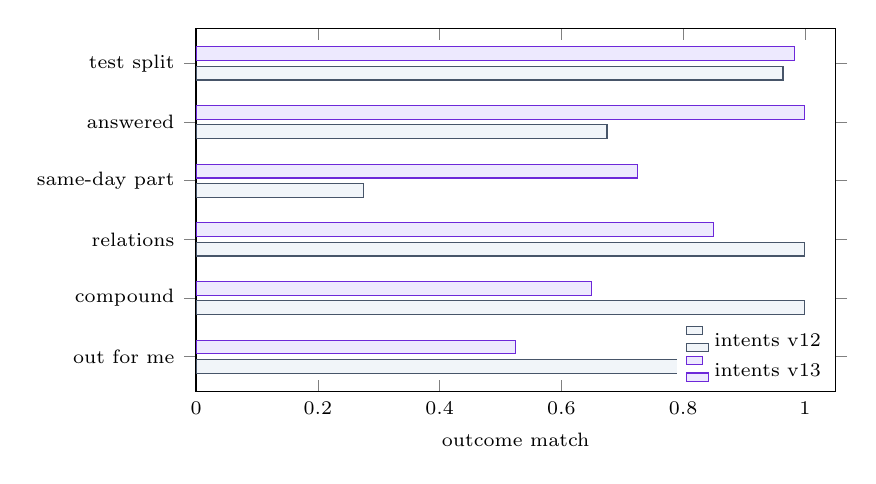
\begin{tikzpicture}
\begin{axis}[
  xbar, bar width=5pt, width=0.8\textwidth, height=6.2cm,
  xmin=0, xmax=1.05, xlabel={outcome match}, xlabel style={font=\scriptsize},
  symbolic y coords={out for me, compound, relations, same-day part, answered, test split},
  ytick=data, tick label style={font=\scriptsize}, enlarge y limits=0.12,
  legend style={font=\scriptsize, at={(1.0,0.0)}, anchor=south east, draw=none, fill=white},
  legend cell align=left]
\addplot[fill=codefill, draw=codeline] coordinates {(0.964,test split) (0.675,answered) (0.275,same-day part) (1.0,relations) (1.0,compound) (0.975,out for me)};
\addplot[fill=modelfill, draw=modelline] coordinates {(0.983,test split) (1.0,answered) (0.725,same-day part) (0.85,relations) (0.65,compound) (0.525,out for me)};
\legend{intents v12, intents v13}
\end{axis}
\end{tikzpicture}
\caption{Adding generators is a trade: v13 learns what its two new generators teach (answered, same-day part) and the
test split improves, but older skills fall.}
\label{fig:abl-suites}
\end{figure}

\subsection{Policy, replies and safety}
\textbf{Retrievers.} Three retrievers find the rules for the policy check: word matching (BM25), dense embeddings,
and the two fused (Figure~\ref{fig:abl-ret}). Each wins somewhere. On requests with the hints the reading adds (a
one-off absence adds ``make-up''), the hybrid is best (93.4\% of correct rules in the top 5). On questions worded
unlike the rules, dense search is best (87.8\%), because it matches meaning, not words. On raw requests without hints,
BM25 is best (77.4\%) and dense search collapses (45.3\%): ``I'm at a conference in week 7'' never mentions make-up
classes, so only the hint can bring that rule in. The hybrid is never far from the best, so the app uses it.

\textbf{The policy model.} Prompted Gemini and the fine-tuned adapter allow or deny almost equally well (98\% and
99\%), but only the adapter learned that a teacher's absence obliges a make-up class: it names that obligation every
time it applies (recall 1.00), where Gemini almost never does (0.21). A rule that is always true in the data is easy
to learn and easy for an instruction-following model to forget.

\textbf{Reply readers.} Four readers turn the same 100 replies into tool calls (Figure~\ref{fig:abl-replies}). The
prompted base model often picks the wrong action (65\%) but fills its arguments correctly; Gemini picks the right
action but gets arguments wrong (85.5\%); keywords fail on counter-offers and vague replies (66\%); the fine-tuned
adapter is right on both counts every time. No reader ever took an unsafe action, because every call is checked.

\textbf{Safety by architecture.} To test whether safety depends on the model, the safety set was run with a parser
that obeys every injected instruction. It still handled 49 of 50 cases safely, with no injection succeeding, no
change made without authority and no private reason revealed: the guarantees come from the pipeline (instructions
removed before reading, authority checked by rule, every change re-solved and approved), not from the model behaving
well.

\begin{figure}[!htb]
\centering
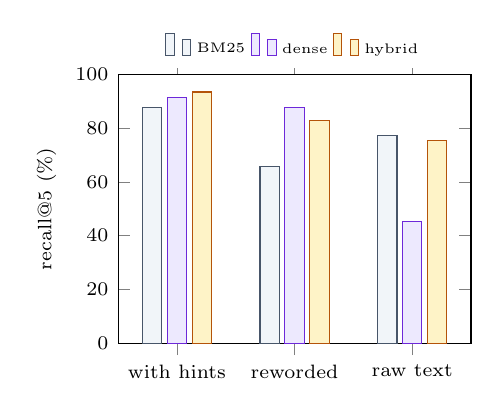
\begin{tikzpicture}
\begin{axis}[
  ybar, bar width=7pt, width=0.5\textwidth, height=5cm,
  ymin=0, ymax=100, ylabel={recall@5 (\%)}, ylabel style={font=\scriptsize},
  symbolic x coords={with hints, reworded, raw text}, xtick=data, tick label style={font=\scriptsize},
  legend style={font=\tiny, at={(0.5,1.02)}, anchor=south, legend columns=3, draw=none}, enlarge x limits=0.25]
\addplot[fill=codefill, draw=codeline] coordinates {(with hints,87.7) (reworded,65.8) (raw text,77.4)};
\addplot[fill=modelfill, draw=modelline] coordinates {(with hints,91.5) (reworded,87.8) (raw text,45.3)};
\addplot[fill=solverfill, draw=solverline] coordinates {(with hints,93.4) (reworded,82.9) (raw text,75.5)};
\legend{BM25, dense, hybrid}
\end{axis}
\end{tikzpicture}\hfill
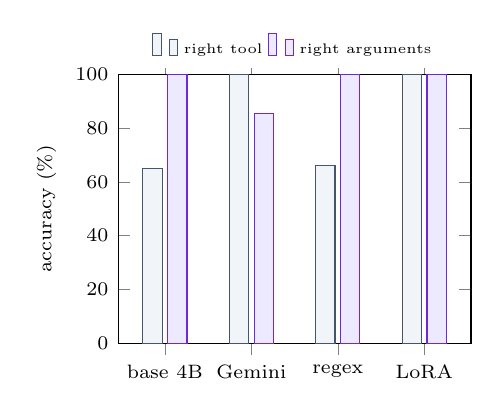
\begin{tikzpicture}
\begin{axis}[
  ybar, bar width=7pt, width=0.5\textwidth, height=5cm,
  ymin=0, ymax=100, ylabel={accuracy (\%)}, ylabel style={font=\scriptsize},
  symbolic x coords={base 4B, Gemini, regex, LoRA}, xtick=data, tick label style={font=\scriptsize},
  legend style={font=\tiny, at={(0.5,1.02)}, anchor=south, legend columns=2, draw=none}, enlarge x limits=0.18]
\addplot[fill=codefill, draw=codeline] coordinates {(base 4B,65) (Gemini,100) (regex,66) (LoRA,100)};
\addplot[fill=modelfill, draw=modelline] coordinates {(base 4B,100) (Gemini,85.5) (regex,100) (LoRA,100)};
\legend{right tool, right arguments}
\end{axis}
\end{tikzpicture}
\caption{Left: rule retrieval by query type; each retriever wins somewhere, the hybrid is never far behind. Right:
reading 100 stakeholder replies; only the fine-tuned adapter gets both the action and its arguments right.}
\label{fig:abl-ret}
\label{fig:abl-replies}
\end{figure}

\begin{table}[!htb]
\centering\small
\begin{tabularx}{\textwidth}{@{}L{3.0cm} L{4.6cm} Y@{}}
\toprule
\textbf{Ablation} & \textbf{Comparison} & \textbf{Result}\\
\midrule
Retriever & BM25 vs dense vs hybrid, recall@5 & With hints: 87.7 / 91.5 / \best{93.4}\%; reworded: 65.8 / \best{87.8} / 82.9\%; raw text: \best{77.4} / 45.3 / 75.5\%\\
Policy model & Prompted Gemini vs fine-tuned 4B & Make-up obligation recall 0.21 vs \best{1.00}; cited deny recall 0.80 vs \best{0.90}\\
Reply reader & Prompted base vs Gemini vs regex vs LoRA & Tool accuracy 65 / 100 / 66 / \best{100}\%; arguments 100 / 85.5 / 100 / \best{100}\%\\
Safety by architecture & Our parser vs a parser that obeys every injection & Still 49/50 safe, \best{0} injection successes\\
\bottomrule
\end{tabularx}
\caption{Policy, reply and safety ablations.}
\label{tab:abl-pol}
\end{table}

\subsection{Timetable questions and memory}
\textbf{A model against a regex.} The regex reader, which the chat falls back to, answers 242 of the 362 single
questions right; prompted Gemini 320; the first fine-tuned lookup adapter 329. Reading what a question asks is
mostly a language problem, and the trained small model handles it best.

\textbf{Reading or memorising?} The same 362 questions were asked in the app's department, in that department with
every teacher's name, the head of department and the course titles shuffled, and in a department the models never saw,
with shared and co-taught courses. Scores barely move (v2: 347, 343, 345; v3: 346, 346, 343), so the adapters read
the question and let code find the names, rather than remembering who is who in one department.

\textbf{Output format: the cleanest ablation.} v3.2 and v4 were trained on \emph{exactly the same rows}, continuing
from the same adapter with the same settings; only the answer's format differs: v3.2 writes v3's flat choices (any
field on any tool, slot numbers, week numbers), v4 writes the lookup vocabulary (a part per thing asked, each tool
with only its own fields, clock times and periods, request parts with their words). Any difference between them is
the format's. On single questions they are alike (339 and 337 of 362). On long and mixed messages v4 is clearly better
(Figure~\ref{fig:abl-format}): 140 whole messages right against 119, 483 of 561 question parts against 445, and 122 of
123 requests found against 117. In the chat it fills ``there'' from the answer in 7 of 8 cases against 5. A typed
vocabulary helps most exactly where messages are long and mixed, because each part is written on its own, with only
the fields its tool has.

\textbf{New data and forgetting.} Against v3, v4 lost 25 single questions and gained 16. The losses are the same few
kinds in every department: ``in week $N$'' read as week $N-1$, ``can I have Thursday free?'' read as a question, ``why
was X's class cancelled?'' looked up instead of kept private. None of them appears in v4's new rows: continuing from
an adapter on new data forgets what the new data does not mention, unless enough of the old rows are replayed.

\textbf{Memory.} The 400 test follow-ups were looked up as typed, and after memory rewrote them: 146 right without
memory, 387--388 with it. Without memory, fewer than four follow-ups in ten work at all. \textbf{Memory v2} fills a
request from the answer in the same message; it depends on the lookup format, since a request part must keep its
words to be filled. \textbf{Plurals}: memory v1 already handles ``these days'' (26/26) and ``those times'' (17/17),
but replaces a person with ``the same time for X'' only 9 times in 21, which is what v1.1's new rows teach.

\begin{figure}[!htb]
\centering
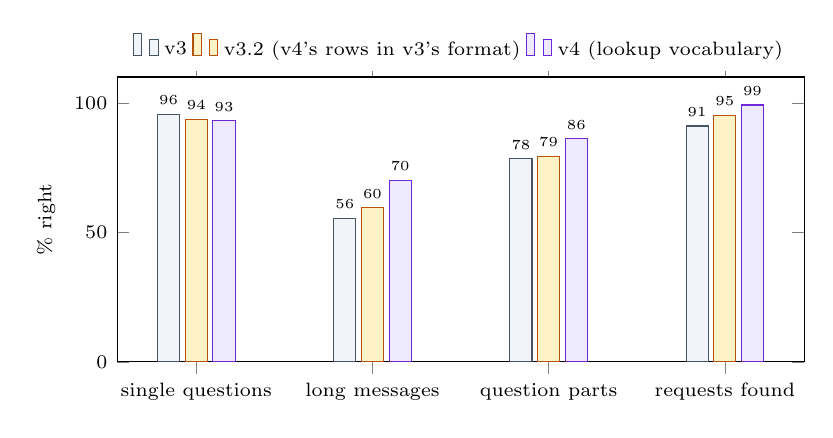
\begin{tikzpicture}
\begin{axis}[
  ybar, bar width=8pt, width=0.85\textwidth, height=5.2cm,
  ymin=0, ymax=110, ylabel={\% right}, ylabel style={font=\scriptsize},
  symbolic x coords={single questions, long messages, question parts, requests found}, xtick=data,
  tick label style={font=\scriptsize},
  legend style={font=\scriptsize, at={(0.5,1.02)}, anchor=south, legend columns=3, draw=none}, enlarge x limits=0.15,
  nodes near coords, nodes near coords style={font=\tiny},
  every node near coord/.append style={/pgf/number format/fixed, /pgf/number format/precision=0}]
\addplot[fill=codefill, draw=codeline] coordinates {(single questions,95.6) (long messages,55.5) (question parts,78.4) (requests found,91.1)};
\addplot[fill=solverfill, draw=solverline] coordinates {(single questions,93.6) (long messages,59.5) (question parts,79.3) (requests found,95.1)};
\addplot[fill=modelfill, draw=modelline] coordinates {(single questions,93.1) (long messages,70.0) (question parts,86.1) (requests found,99.2)};
\legend{v3, {v3.2 (v4's rows in v3's format)}, {v4 (lookup vocabulary)}}
\end{axis}
\end{tikzpicture}
\caption{The output-format ablation. v3.2 and v4 differ only in format; the typed vocabulary gains most on long and
mixed messages.}
\label{fig:abl-format}
\end{figure}

\begin{table}[!htb]
\centering\small
\begin{tabularx}{\textwidth}{@{}L{3.0cm} L{4.6cm} Y@{}}
\toprule
\textbf{Ablation} & \textbf{Comparison} & \textbf{Result}\\
\midrule
Model vs regex & Regex vs Gemini vs lookup v1 (set A) & 242 vs 320 vs 329 of 362\\
Memorisation & The same questions in the app's, a shuffled and an unseen department & v2: 347 / 343 / 345; v3: 346 / 346 / 343\\
\textbf{Output format} & v3.2 vs v4: \emph{the same training rows}, flat choices vs the lookup vocabulary & Long messages 119 vs \best{140}; requests found 117 vs \best{122}; single questions alike (339 vs 337)\\
New data, forgetting & v3 vs v4 on single questions & v4 lost 25 and gained 16 on set A\\
Memory & Without vs with memory (400 follow-ups) & 146 vs \best{387--388} looked up right\\
Memory v2 & v3.2 vs v4 request parts & 5/8 vs \best{7/8} chat cases\\
Plurals & Memory v1 on three kinds of plural & 26/26, 17/17, 9/21\\
\bottomrule
\end{tabularx}
\caption{Timetable-question and memory ablations.}
\label{tab:abl-chat}
\end{table}

\subsection{Coordinator agent}
\textbf{Fine-tuning.} On the 19-family suite the prompted 4B base passes 66.7\%, Gemini 85.1\% and the fine-tuned agent
100\% (Figure~\ref{fig:abl-agent}). The agent learns from its own verified trajectories: which tool to call, in what
order, and when to stop.

\textbf{SFT against SFT followed by DPO.} DPO trains on pairs of a better and a worse episode of the same request. On
the full 49-family suite v7 scores 79.0\% after SFT and 77.8\% after DPO, a difference within the noise of two runs of
the same job (up to 10 episodes in one family). Its held-out preference accuracy was only 0.65 on 48 pairs: with a
few hundred pairs from one source, DPO barely moved the model.

\textbf{Epochs.} Validation loss shows that a second epoch helps a little and a third never does; more episodes help
more than more passes.

\textbf{Code fixes against more training.} Five families failed for reasons in the tools, not the model (a daily cap
on teaching days, for example). Fixing the tools took those families from 24 to 47 of 50 without retraining; the
exam-week family went from 0 to 9--10 of 10 once the agent could read the examination regulations. When a model keeps
failing at something, the cause is often in its tools or inputs, and code is the cheaper fix.

\begin{figure}[!htb]
\centering
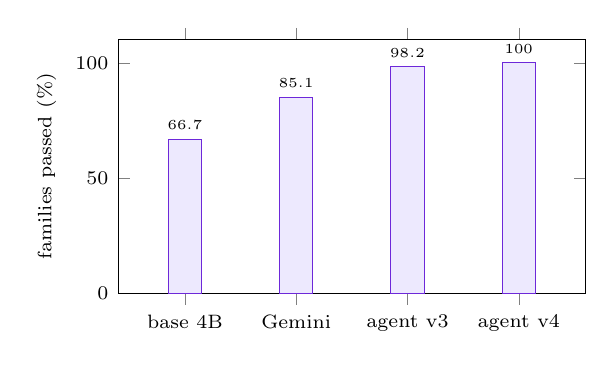
\begin{tikzpicture}
\begin{axis}[
  ybar, bar width=12pt, width=0.62\textwidth, height=4.8cm,
  ymin=0, ymax=110, ylabel={families passed (\%)}, ylabel style={font=\scriptsize},
  symbolic x coords={base 4B, Gemini, agent v3, agent v4}, xtick=data, tick label style={font=\scriptsize},
  enlarge x limits=0.2, nodes near coords, nodes near coords style={font=\tiny},
  every node near coord/.append style={/pgf/number format/fixed, /pgf/number format/precision=1}]
\addplot[fill=modelfill, draw=modelline] coordinates {(base 4B,66.7) (Gemini,85.1) (agent v3,98.2) (agent v4,100)};
\end{axis}
\end{tikzpicture}
\caption{The coordinator agent on the 19-family default suite: fine-tuning a 4B model on verified trajectories beats
a much larger prompted model.}
\label{fig:abl-agent}
\end{figure}

\begin{table}[!htb]
\centering\small
\begin{tabularx}{\textwidth}{@{}L{3.0cm} L{4.6cm} Y@{}}
\toprule
\textbf{Ablation} & \textbf{Comparison} & \textbf{Result}\\
\midrule
Fine-tuning & Base 4B vs Gemini vs SFT (19 families) & 66.7\% vs 85.1\% vs \best{100\%}\\
SFT vs SFT + DPO & v7 SFT vs v7 DPO (49 families $\times$ 10) & 79.0\% vs 77.8\%: within noise\\
Epochs & Epoch 1 vs 2 vs 3 & The second helps little, the third never\\
Code fixes vs training & v7 SFT with and without five tool fixes & Those five families 24/50 $\to$ \best{47/50}\\
Policies & With vs without the exam regulations & Exam-week family 0/10 $\to$ 9--10/10\\
\bottomrule
\end{tabularx}
\caption{Agent ablations. Two runs of the same job differ by up to 10 episodes in one family: differences under
that are noise.}
\label{tab:abl-agent}
\end{table}

\subsection{What the ablations show overall}
Across all five areas the same pattern appears. \textbf{Where code can decide, code should}: verified offers beat
invented ones, names resolved by code made training seven times cheaper at no cost, the safety guarantees held even
with a parser that obeys every injection, and tool fixes did what more training had not. \textbf{Where language must
be read, a small model trained on the task beats a large one told about it}, in reading requests, policy obligations,
replies, timetable questions and agent behaviour. \textbf{What remains is mostly about data}: new rows dilute old
skills, continued training forgets what new data omits, and the ledger cannot show its effect on single-conflict
scenarios. Each of these points to a change in data or benchmark, not in the architecture.

% ==================================================================
\section{Limitations}
\label{sec:limits}
% ==================================================================
\begin{itemize}
\item \textbf{H4 is not supported.} With one conflict per scenario the ledger has little to act on; scenarios with a
sequence of requests among the same people are needed.
\item \textbf{Mixed models in the main comparison.} Ours runs on the fine-tuned 4B model, the baselines on the larger
Gemini; a run with the same model on both sides would separate the method from the model.
\item \textbf{Human validation.} Explanation faithfulness and the judge are measured automatically, not yet against
human ratings, and the faculty pilot waits for ethics clearance.
\item \textbf{Synthetic data and simulated people.} Every dataset is generated or team-written, the handbook is a
stand-in, and negotiation partners are simulators with four styles; real people may behave otherwise.
\item \textbf{Training-data gaps.} No training row asks about a \emph{range} of times (``between 10 and 2'') or dates,
so every lookup adapter reads only the ends; typed date-range requests (``cancel all my classes from 9 to 13 Nov'')
are asked back, since the request vocabulary holds weeks, not dates (the click-based range builder handles them).
Continuing an adapter forgets what its new rows do not mention unless enough old rows are replayed (v4 and
``in week $N$''), and adding generators can cost older skills (v13's compound requests).
\item \textbf{Linear attention not adapted.} The adapters' layer pattern misses Qwen3.5's 24 linear-attention layers;
adapting them is untested.
\item \textbf{Infrastructure.} One shared GPU server; when it is unreachable the rule-based stand-ins are much weaker
(51.6\% against 96.4\% on reading requests).
\end{itemize}

% ==================================================================
\section{Conclusions}
% ==================================================================
Letting the solver define what may be offered, and the language model only explain it and read the answers, settles
infeasible timetable requests more often and far closer to the best possible outcome than letting a model invent
options, even with the same solver filtering them: 89.4\% against 75.6\%, an oracle gap of 0.04 against 0.63, and not
one infeasible offer. The same division of labour carries through the system: small fine-tuned adapters read
language into typed vocabularies and beat a much larger prompted model on every reading task, while code resolves
names, dates and rules and answers every question from the timetable. The ablations locate what remains: the ledger
needs longer histories to show its effect, grounded explanations are what keep private reasons private, and most
reading errors trace to gaps in generated training data rather than to the architecture, which points to the next
step: training data drawn from real requests.

% ==================================================================
\section*{Reproducibility}
% ==================================================================
\small
Every dataset is generated from fixed seeds, with its answers known by construction. The whole system runs offline
on its deterministic stand-ins, and its tests need no model or API key. Every model answer is cached by model and
prompt, so every table can be scored again without calling a model, and interrupted runs resume. The adapters are
trained on free Kaggle GPUs from the same data, and served with \texttt{llama-server} on one base model.
\normalsize

% ==================================================================
\begin{thebibliography}{9}
\small
\setlength{\itemsep}{2pt}

\bibitem{burke2002} E.~K.~Burke, S.~Petrovic. Recent research directions in automated timetabling.
\emph{European Journal of Operational Research}, 140(2):266--280, 2002.

\bibitem{hu2022} E.~J.~Hu, Y.~Shen, P.~Wallis, Z.~Allen-Zhu, Y.~Li, S.~Wang, L.~Wang, W.~Chen. LoRA: Low-rank
adaptation of large language models. \emph{ICLR}, 2022.

\bibitem{kambhampati2024} S.~Kambhampati et al. Position: LLMs can't plan, but can help planning in LLM-Modulo
frameworks. \emph{ICML}, 2024.

\bibitem{lewis2020} P.~Lewis et al. Retrieval-augmented generation for knowledge-intensive NLP tasks.
\emph{NeurIPS}, 2020.

\bibitem{liffiton2008} M.~H.~Liffiton, K.~A.~Sakallah. Algorithms for computing minimal unsatisfiable subsets of
constraints. \emph{Journal of Automated Reasoning}, 40(1):1--33, 2008.

\bibitem{ortools} L.~Perron, F.~Didier. CP-SAT. Google OR-Tools, \url{https://developers.google.com/optimization}.

\end{thebibliography}

\end{document}
